% Chapter 4

\chapter[Implementation and on-sky testing]{\setstretch{1}Implementation and on-sky testing} % Main chapter title
\label{chap:implementation}

\epigraph{\setstretch{1}\small\itshape Ever tried. Ever failed. No matter. \\ Try again. Fail again. Fail better.}{S. Beckett}

\section{Key pre-flight procedures}
\subsection{Inertia measurement}
While CAD models allowed to us to estimate the moment of inertia of the payload, this is only an approximation. For testing and for launch, the payload will be different than the model we have: we will either miss some components because they are not yet installed, or have additional components such as the ballasts, the crush pads, or the weights that are used to balance the payload.

We use a simple procedure to estimate the moment of inertia about $\vectors{z}_\gyro$ of the payload while hanging from a crane. For this purpose, we command the CCMG to input a torque to the payload by moving the gimbal at a constant velocity. According to Eq.~\ref{eq:CCMGTorque}, $\ccmgtorque =  20.8\times \dot{\theta}\cos\theta$. According to conservation of angular momentum, the rate of change of the total angular momentum about $\vectors{z}_\gyro$ is $(\inertia\dot{\gyroVec})_\vectors{z} = \ccmgtorque = 20.8\times \dot{\theta}\cos\theta$.

We measure the inertia $\inertia_\vectors{z}$ by averaging measurements of the angular acceleration $\dot{\gyroVec}_\vectors{z}$, divided by the instantaneous input torque, which is numerically more stable than averaging its inverse since the accelerations, expressed in \si{\radian\per\second} are typically very small. A measure of the inertia is then the inverse of this average. We consistently measure an inertia of roughly \SI{1700}{\kilo\gram\raiseto{2}\meter}, which is about 15\% higher than the expected CAD model estimates. This reflects some errors in assigning the proper masses in the CAD model.


\subsection{Sensor alignment and calibration}
While the intrinsic noise of our sensors has been characterized in Section~\ref{chap:controls}.\ref{subsec:gyros}, it is important to test them while mounted to the payload, align their axes to the other reference frames, and study their spectral energy distribution. Mounting the gyroscopes in a 3-dimensional mount on the truss will inevitably lead to alignment errors and the contribution of new vibration frequencies present in the structure and excited by the moving parts on the payload.


\subsubsection{Gyroscope spectral analysis in flight configuration}

The gyroscopes were characterized in quiet laboratory environment that was designed for precision optical interferometry, with special foundations to prevent vibrations being transmitted through the ground. This allowed us to measure the gyroscopes down to their noise levels. However, as soon as we attach the gyroscopes to any structure, the gyroscopes measure their mount's vibration modes. 

%\begin{figure}[!h]
%\begin{center}
%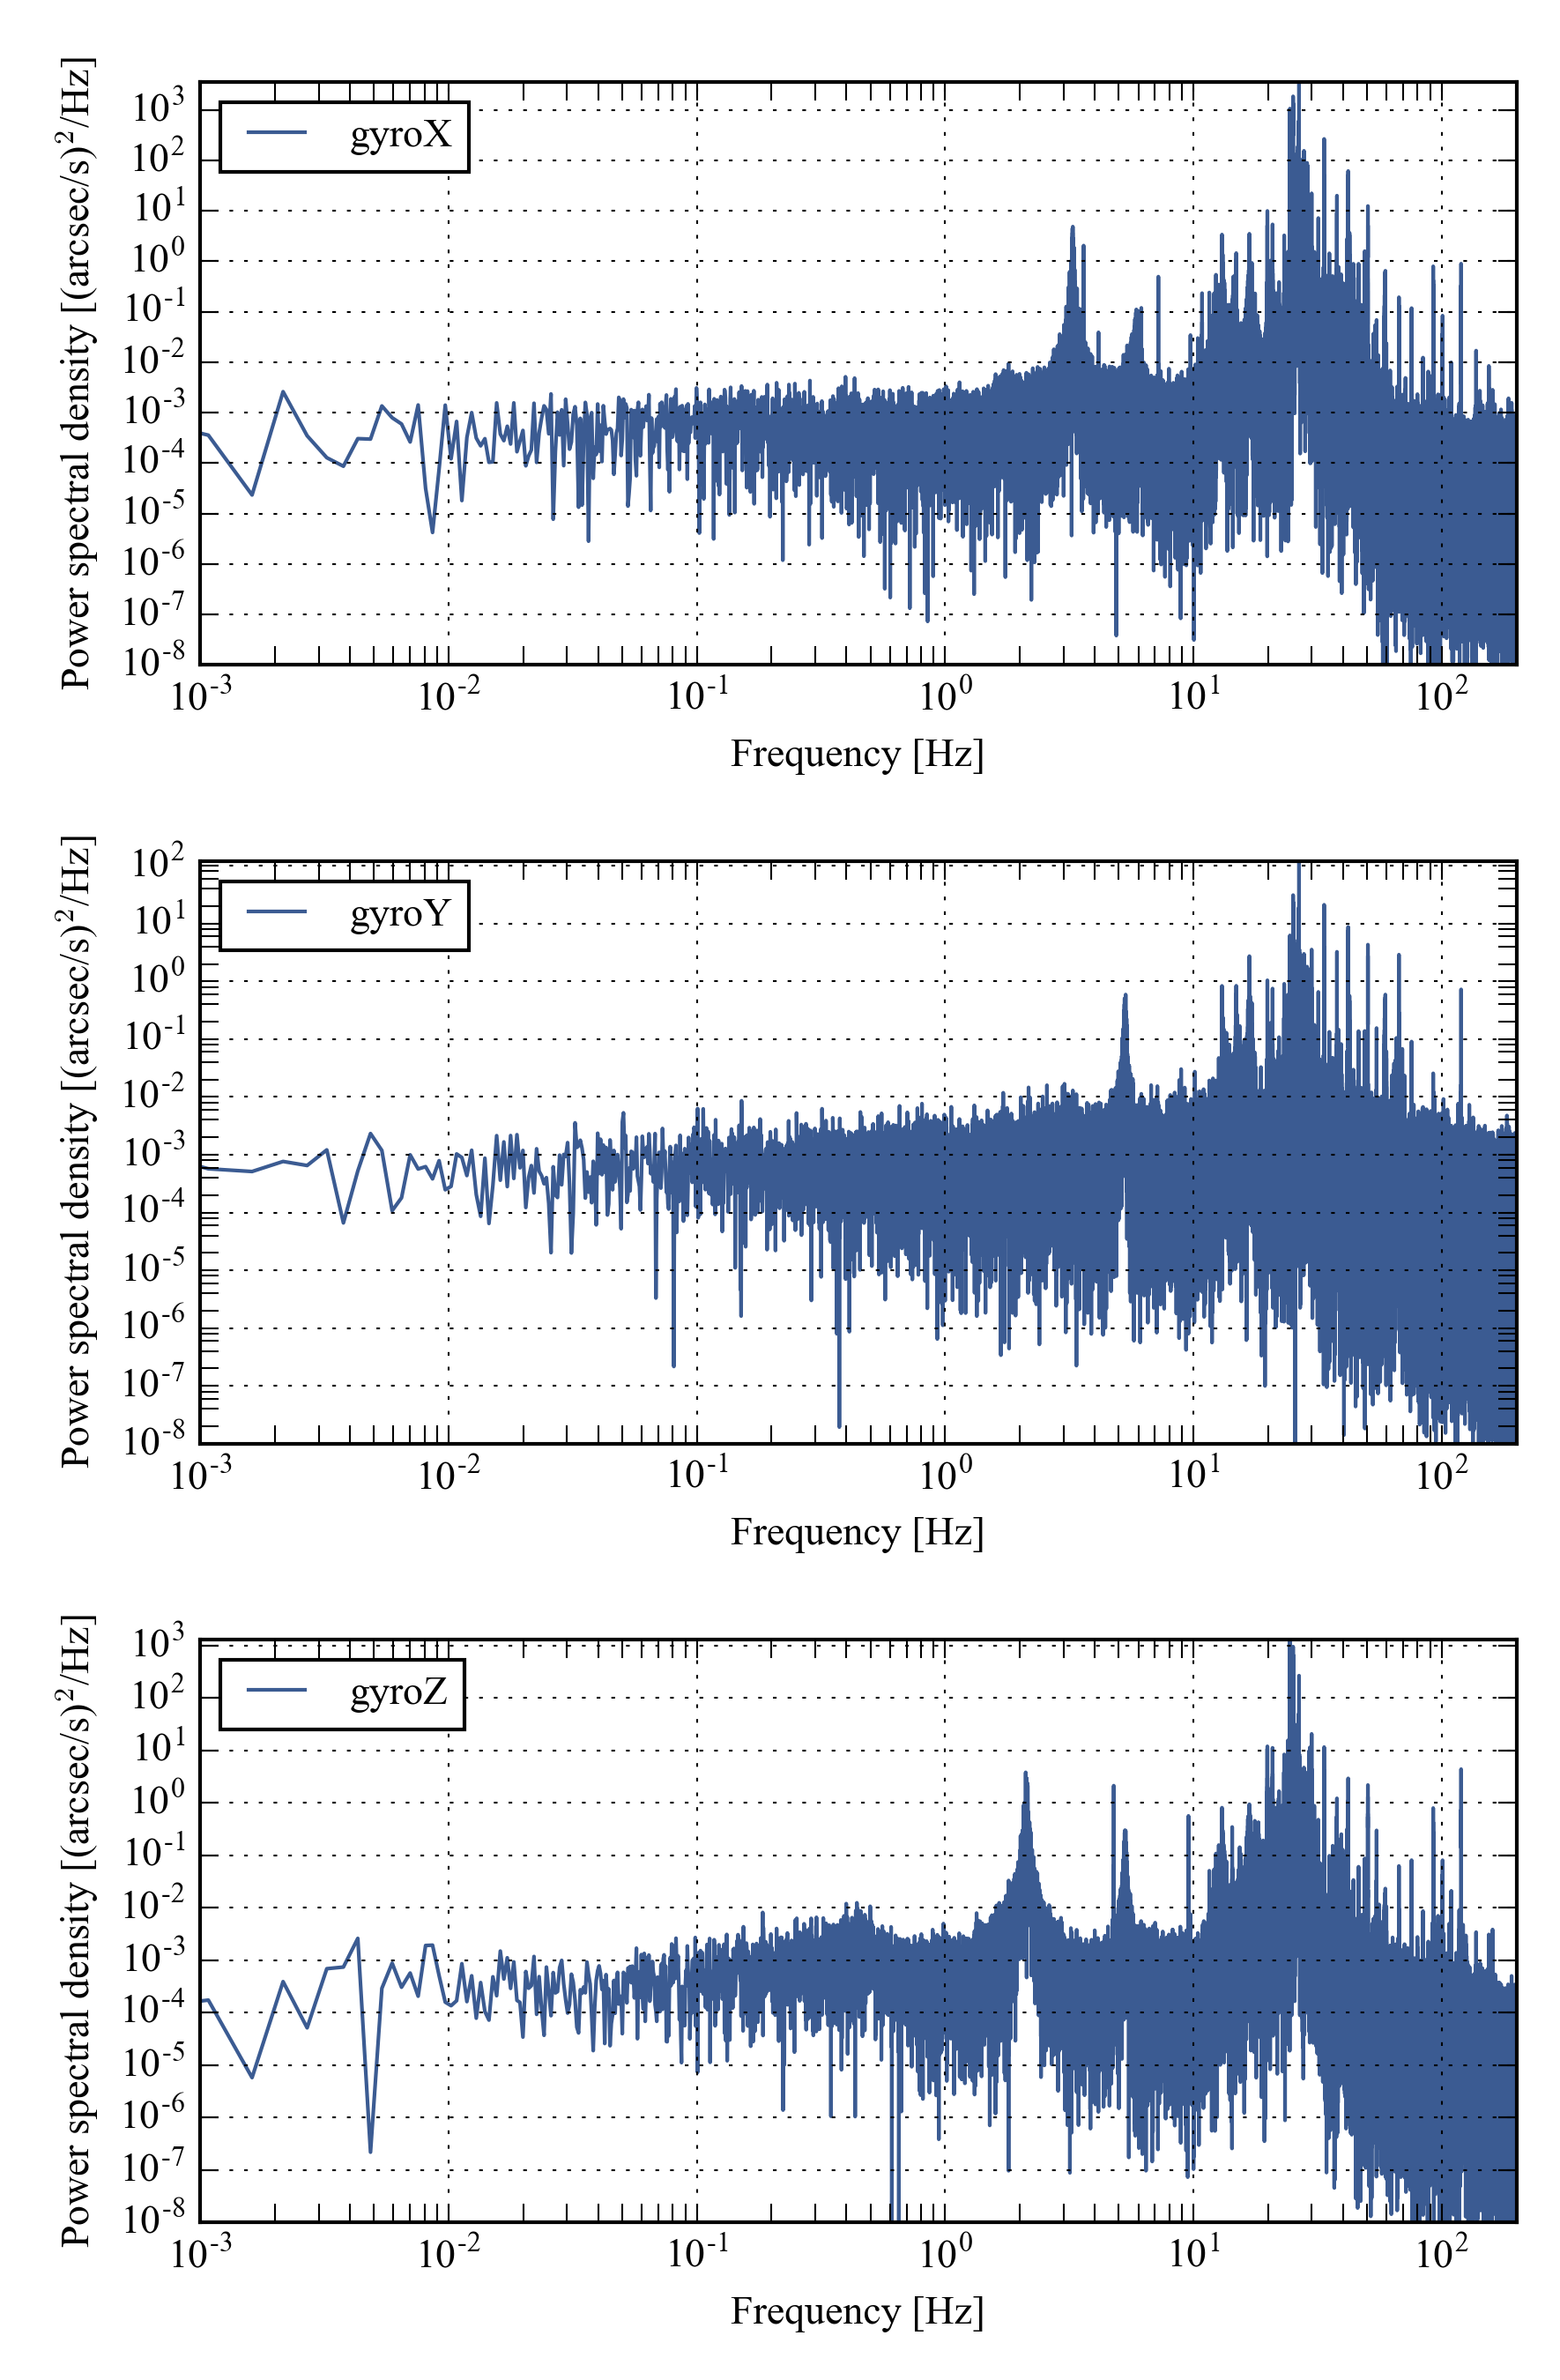
\includegraphics[width=\textwidth]{Figures/multiPSD400.png}
%\label{fig:multiPSD400}
%\vspace{-0.5cm}
%\caption[Gyro PSD with payload on the ground]{Gyro PSD with payload on the ground}
%\end{center}
%\end{figure}


\begin{landscape}
\vspace{-1cm}
\begin{figure}[!h]
\begin{subfigure}[b]{0.7\textwidth}
		\centering
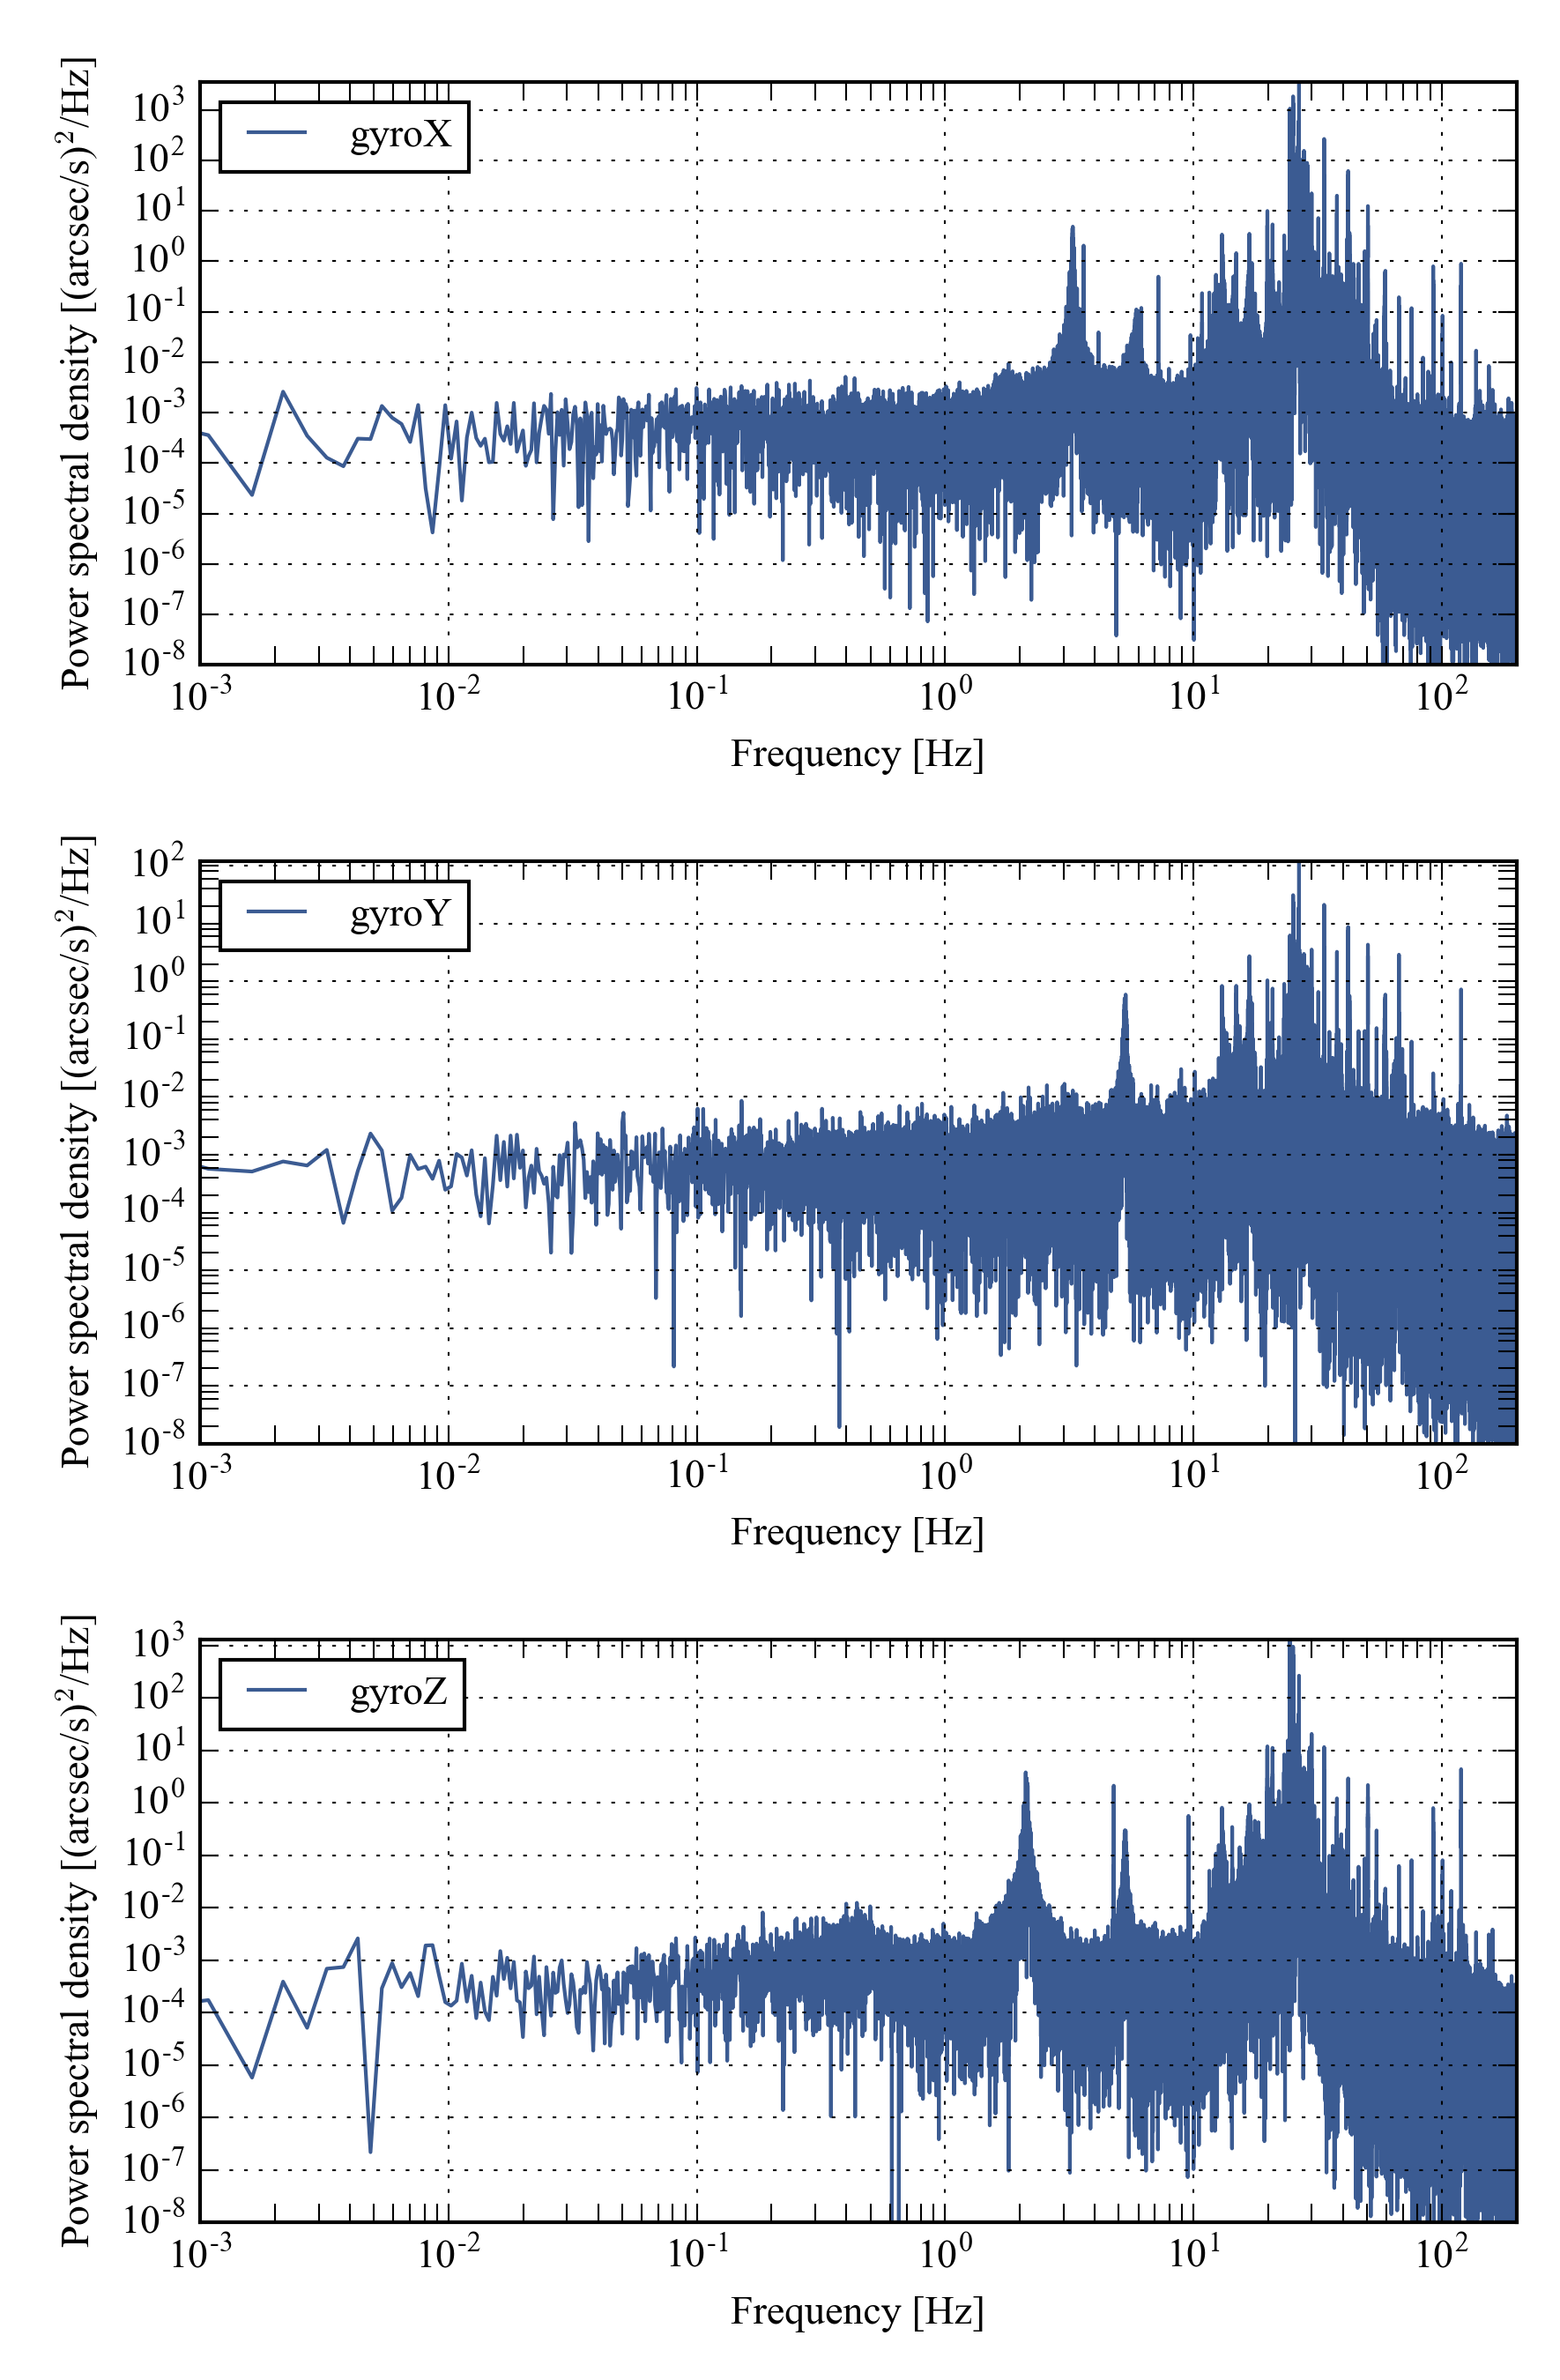
\includegraphics[width=\textwidth]{Figures/multiPSD400.png}

\vspace{-0.5cm}
	\caption{}
	\label{fig:multiPSD400}
	\end{subfigure}
\begin{subfigure}[b]{0.7\textwidth}
		\centering
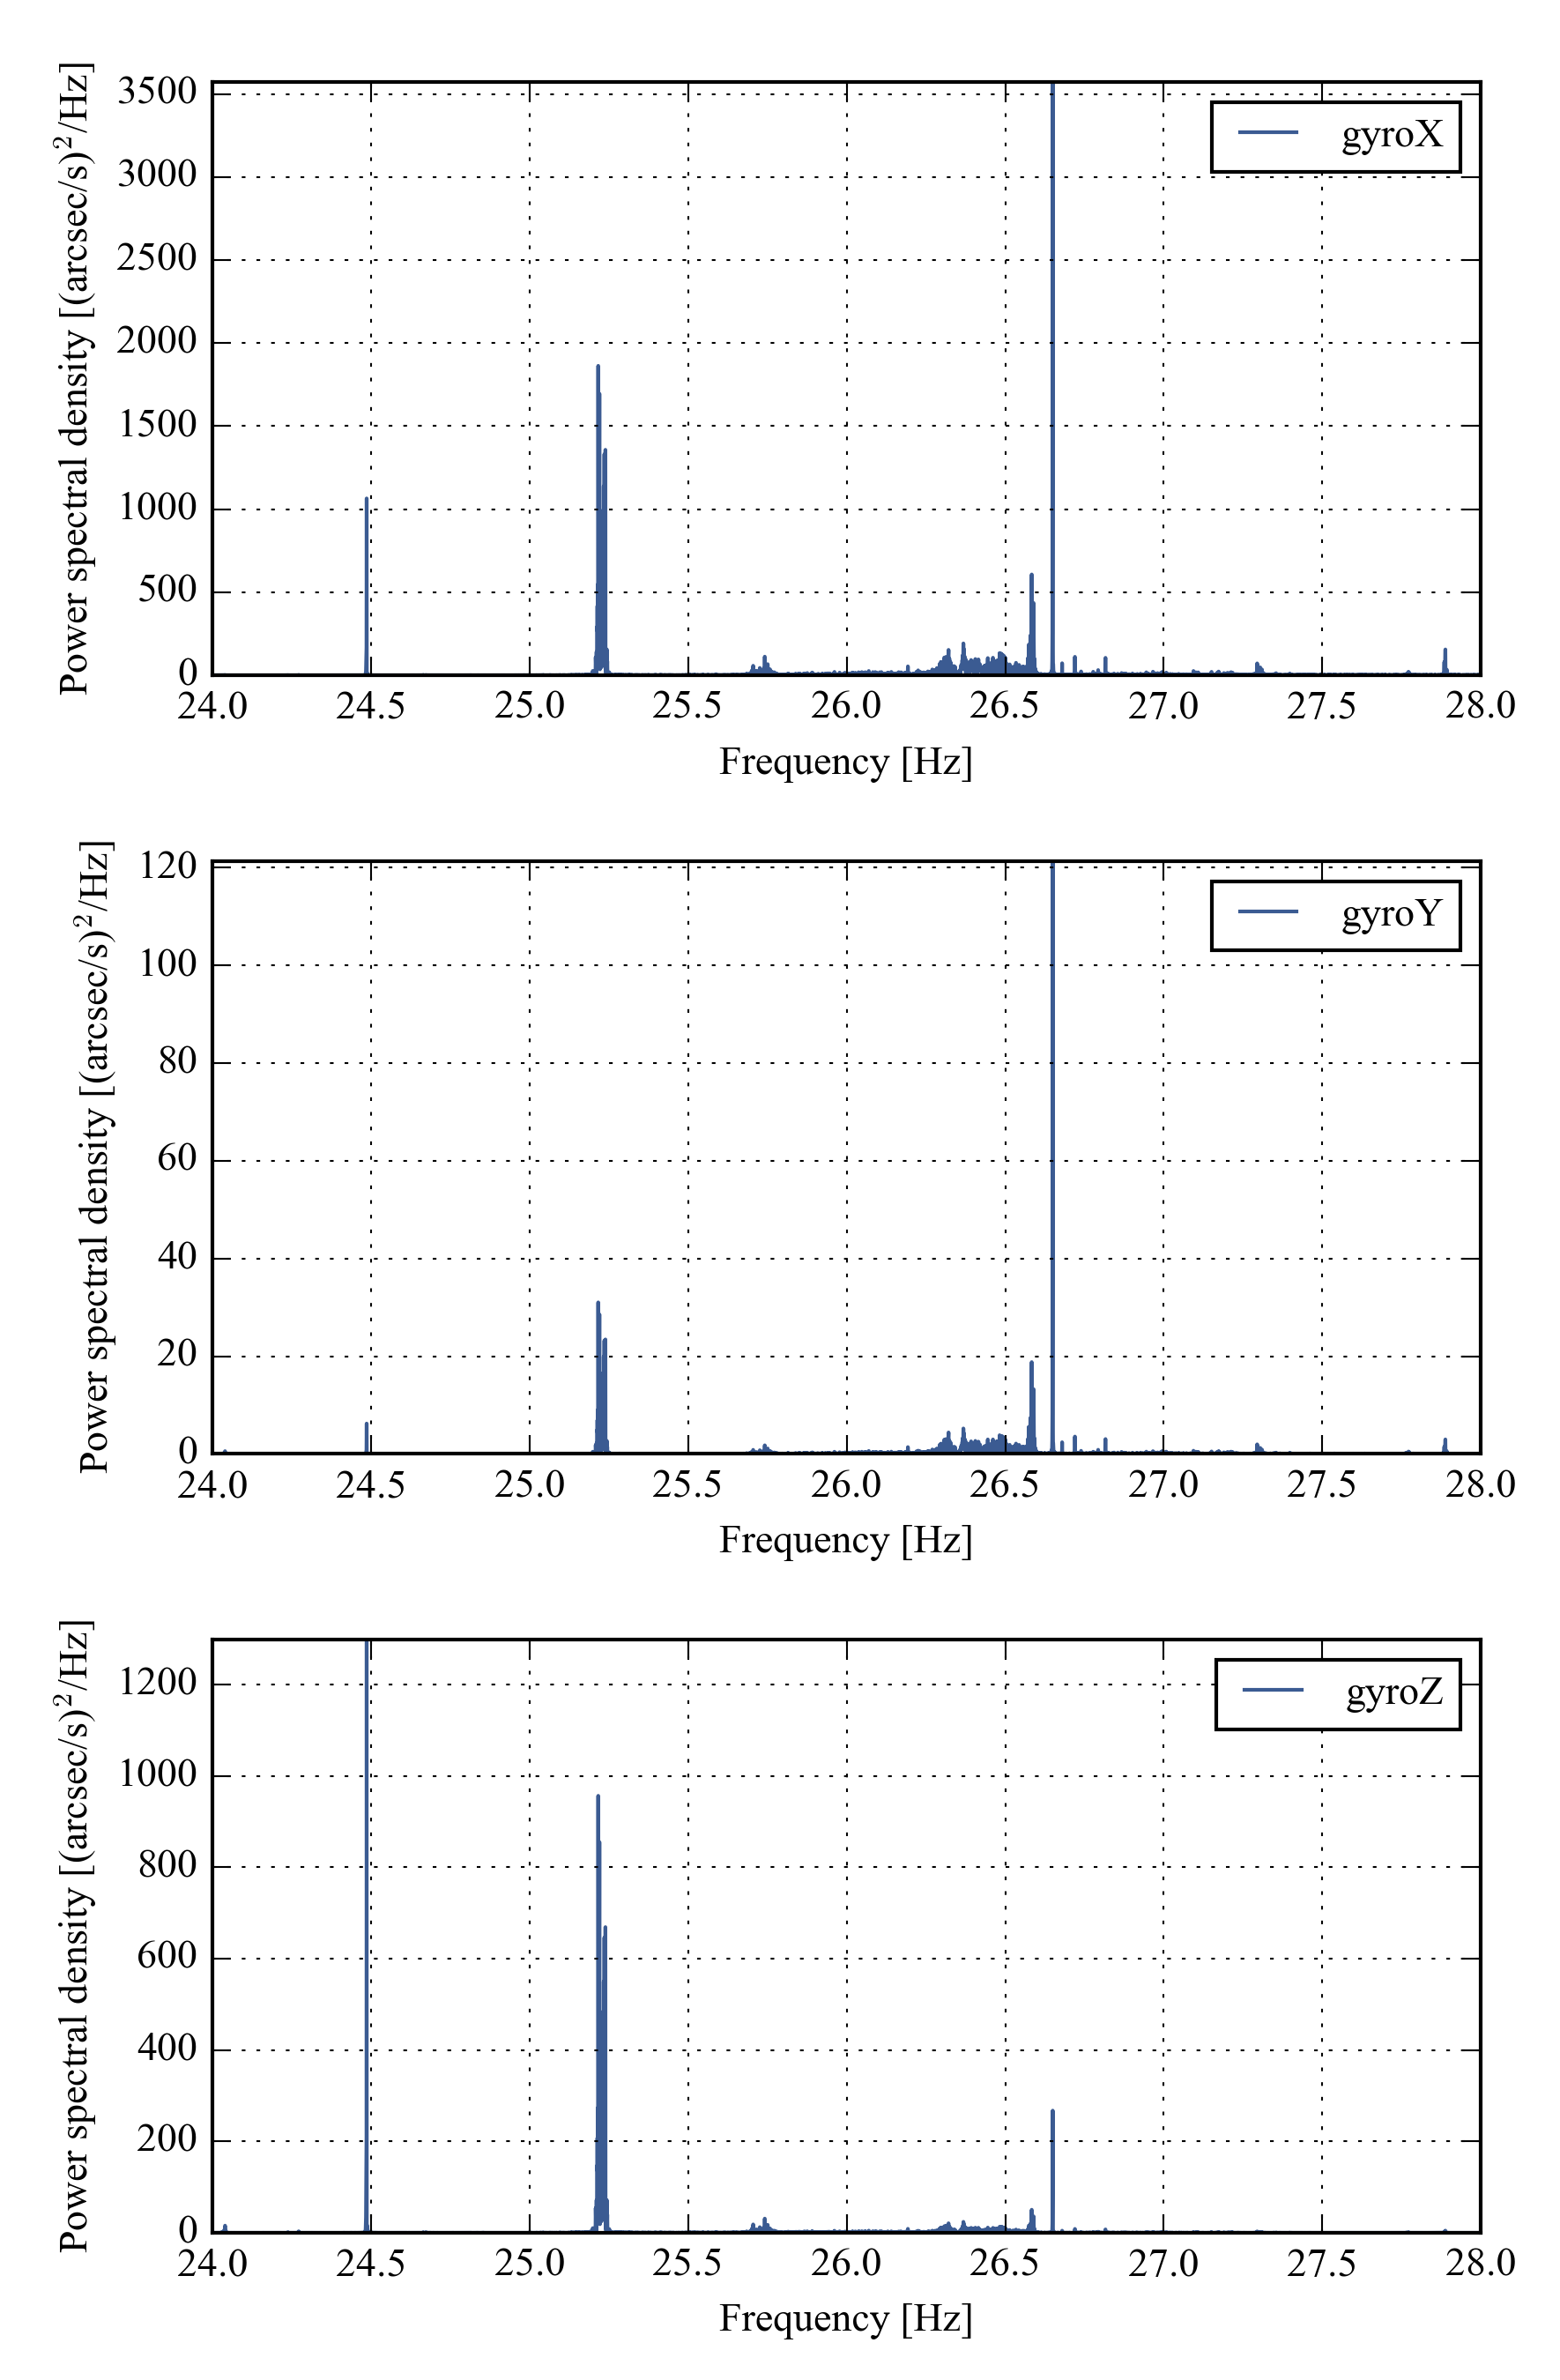
\includegraphics[width=\textwidth]{Figures/multiPSD_no_loglog_zoom_400.png}

\vspace{-0.5cm}
\caption{}
\label{fig:multiPSD400_no_loglog_zoom_400}
	\end{subfigure}
	\vspace{-0.5cm}
\caption[Gyroscope noise]{Gyroscope noise}
\end{figure}
\end{landscape}



We estimate that, once in the box and attached onto the truss, the gyroscope has $\sim$20 times its natural noise levels. Looking at the power spectral density of the velocity time series (Fig.~\ref{fig:multiPSD400}), almost all of the noise power is contained in three strong and sharp peaks, which coincide with the expected first resonant modes of carbon fiber truss structure, obtained through finite element analysis. These modes are precisely located at 24.49, 25.23 and \SI{26.7}{\hertz} with the mass configuration of the time the data was taken, which omits the large siderostat mirrors on each end (Fig.~\ref{fig:multiPSD400_no_loglog_zoom_400}).

The positive conclusion is that the truss has its first resonant frequencies precisely where they were designed to be from CAD modeling, and they are above \SI{20}{\hertz}, which is out of the bandwidth of the attitude control. This noise can then be drastically attenuated either by notch filters (if the frequencies do not shift) or by low-pass filters with a break frequency at a few Hertz. For example at \SI{2.5}{\hertz}, a single-pole low-pass Butterworth filter would attentuate these peaks by \SI{20}{\decibel}, or an attenuation factor of 100. 

One less encouraging result is that these modes do not seem to damp, which means that they are continually being excited. One of the ideas behind bringing the first resonant frequencies above \SI{20}{\hertz} was to have low amplitudes and relatively fast damping. We hypothesize that the truss vibrational modes are excited by the ambient vibration spectrum coming from the air, in particular from the A/C unit.

Examining the PSD in Fig~\ref{fig:multiPSD400}, we also notice some broad peaks at 3, 5.5, and \SI{2}{\hertz} for the x, y, and z axes respectively. These are attributed to motions of the truss within the gondola about the vibration isolators that were installed to decouple the two mechanical structures. 

%\begin{figure}[!h]
%\begin{center}
%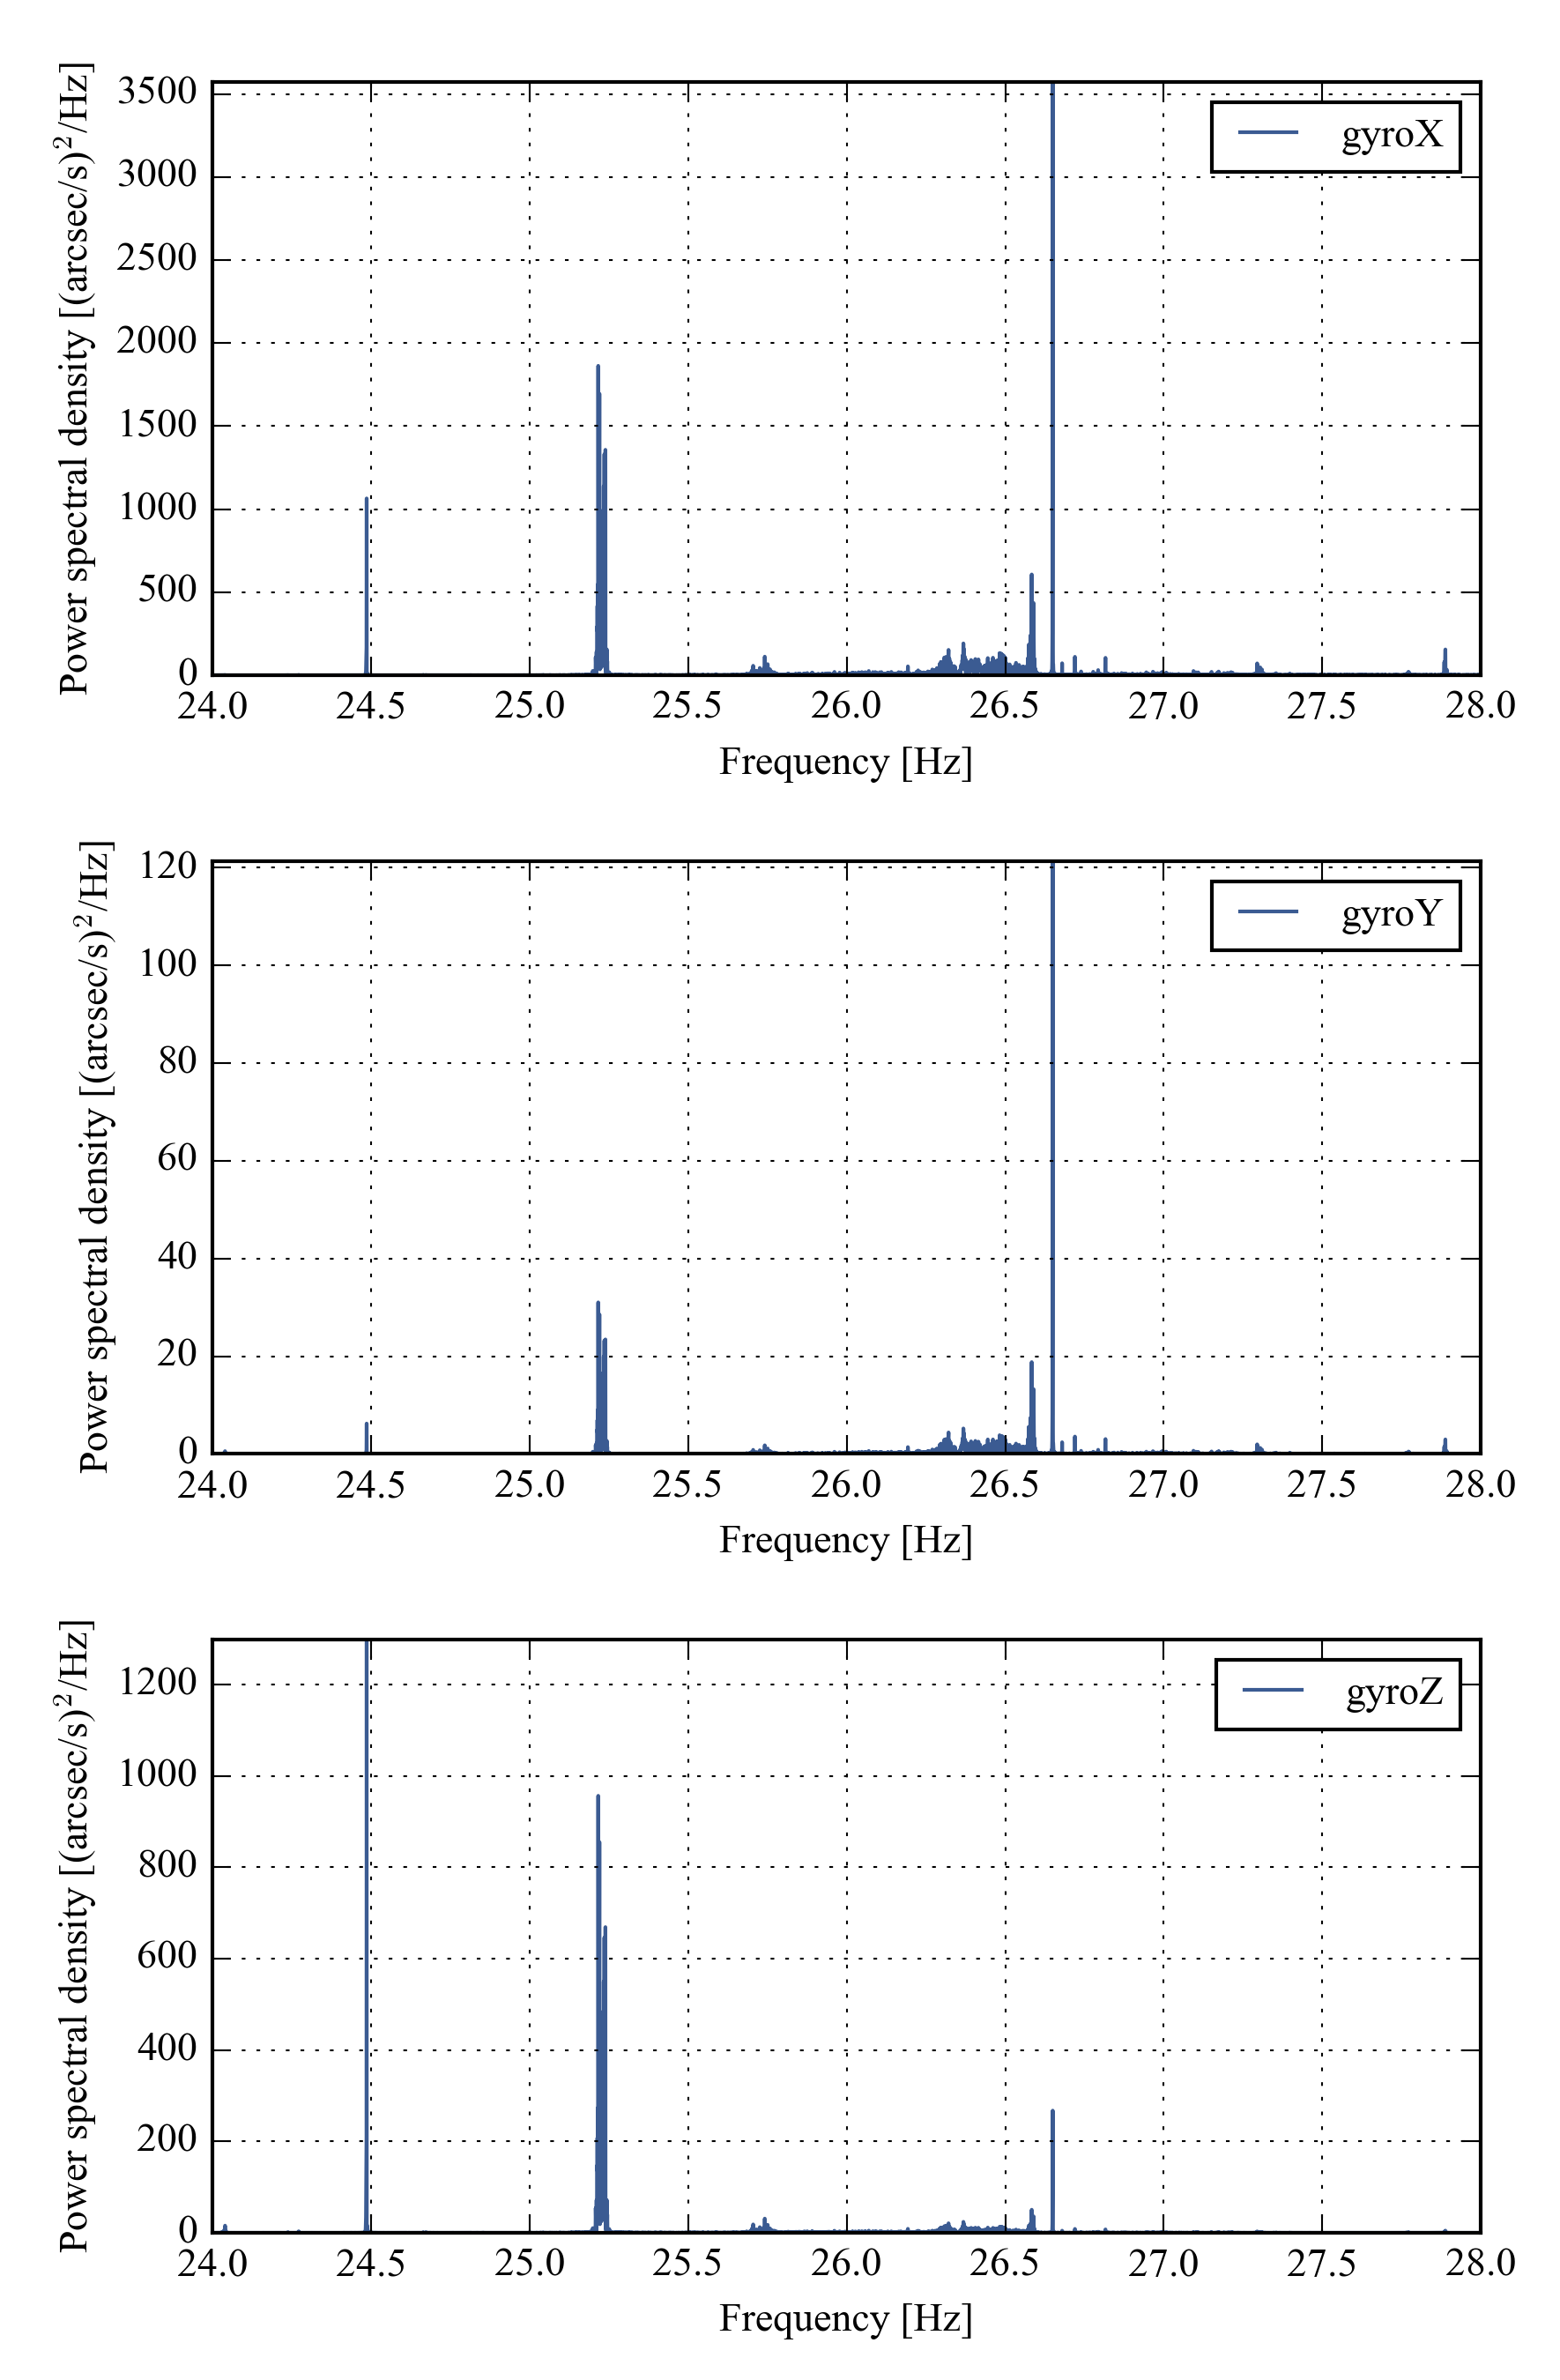
\includegraphics{Figures/multiPSD_no_loglog_zoom_400.png}
%\label{fig:multiPSD400_no_loglog_zoom_400}
%\vspace{-0.5cm}
%\caption[Gyro PSD with payload on the ground - Main peaks]{Gyro PSD with payload on the ground - main peaks.}
%\end{center}
%\end{figure}



\subsubsection{Orthogonalization of gyroscope mount}
\label{ap:gyroOrth}

An orthogonalization procedure was established to determine the correction matrix to apply to the gyroscope velocity vector to make sure measurement were independent from one another. The procedure involves spinning the 3-axis gyroscope mount on one of the rotation stages that we use for flight (which are used for elevation control). 

The system to solve is:
\begin{equation}
\gyroVec^\textrm{meas} = \begin{bmatrix} M_x & m_{xy} & m_{xz} \\   m_{yx} & M_y &m_{yz} \\  m_{zx} & m_{zy} & M_z \end{bmatrix} \gyroVec^\textrm{true} = M \gyroVec^\textrm{true} 
\end{equation}

The 9 matrix elements can be found by commanding the 3-axis mount to rotate at a known velocity about each axes. Hence, by knowing the vector $\gyroVec^\textrm{true}$ (one component is the commanded velocity and the two others are zero) and measuring the velocities on the three axes, we can determine the matrix element for the column corresponding to the current spin axis. 

The gyroscopes are so sensitive that they measure the rotation of the Earth accurately. This corresponds to a bias in the commanded velocity. To mitigate this issue, we spin the 3-axis mount in two opposite directions. The perceived difference in the velocities corresponds to the Earth velocity about that axis. 

Because of cabling constraints, we are only able to spin the 3-axis mount for small angles. This method works very well when the gyroscope can spin freely and do \SI{360}{\degree} rotations, since a lot of the systematics of the setup will cancel out after multiple revolutions. Unfortunately, we do not have access to a state-of-the-art rotation table with a slip-ring.

The matrix we obtain suggests typical alignment errors on the order of 0.1-0.3\%, which correspond to angular errors of a few degrees. While the measurements appear to be repeatable, we noticed that the sum of the squares of the velocities was typically 2\% off from its expected value, which we know since it corresponds to the square of the Earth's rotation velocity. Further, this error varies with different orientations of the gyroscope mount. The typical errors that are seen are consistent with a residual misalignment of a few tenths of degrees between the gyroscopes - a considerable amount.

This could lead to multiple interpretations. First, it is possible (even likely) that the mount deforms under its own gravity in different ways depending on its orientation. Unfortunately, it is not simple to proceed to this orthogonalization method with the mount in its flight orientation, and would require some ground support equipment (GSE) not available at the moment. 

A second possible interpretation is that the gyroscope internal scale factor is changing. We noted that the temperature of the gyroscopes was increased by about \SI{5}{\degreeCelsius} when they are inside the mount on the thermal isolators. This can potentially change their scale factor (which effectively multiplies the measured velocity) as a result of the fiber optics' length changing slightly. 

The path forward towards orthogonalization of the mount is to use a ROMER metrology arm to measure the relative position of the mount faces to within a few arcminutes, when the gyroscopes are in their flight configuration. This would allow us to find the components of the matrix $M$ for the mount on the payload in its final flight configuration. It will also allow us to precisely align the mount to the other important reference frames, such as the star camera reference frame and the telescope reference frame.

The scale factor on the $\vectors{z}$ gyroscope can also be precisely determined if the payload if aligned horizontally with precision. Because of the size of the payload, a good lever arm provides an accurate measure of its horizontal position. The gyroscope on the $\vectors{z}$ axis can thus be aligned with the gravity vector precisely, at which point the expected angular velocity is known, and the scale factor correction can be determined.


\subsubsection{Alignment of gyroscope mount to star camera mounts}

Once the gyroscope is orthogonalized, it remains to be properly referenced to the star camera mount. In fact, because those two key elements of the control system are thermally separated, it is possible that they drift between one another. 

For this purpose, we developed a variant to the traditional Kalman filter described in Chapter~\ref{chap:controls}, which instead of estimating the bias, estimates the rotation matrix between the gyroscope mount and the star camera, as explained in \ref{subsec:enhancedKalman}. Running this filter can be done seamlessly, even in flight, since the number of unknowns is the same as the flight model which estimates bias drifts. 







\subsection{Star camera}

\subsubsection{Tuning tests}

We proceeded to multiple stages of tuning for the star camera, spanning many nights over the past year. In this section, we propose an small excerpt of the data acquired during one night when we varied the exposure time of the camera, to determine the most suitable value for flight. We list here (Table~\ref{tab:starCameraTests}) five experiments starting with an exposure time of \SI{250}{\milli\second} and decreasing the exposure time down to \SI{31}{\milli\second}. During these tests, we compute some statistics on the observations, and are most interested in the success rate, which is the ratio of solutions found over the total number of images taken. By computing these statistics from the outputs of the star camera software, we also noted that the fitted exposure time, which corresponds to the best fit between the known star brightness and the measured camera digital counts, was remarkably accurate when solutions were found. In addition, on the occasion when a false positive was found (that is a solution that is not correct), the exposure time was, predictably, very inaccurate. We decided to add this fitted exposure time information as an additional metric to determine the accuracy and reliability of the star camera software. From the results, we determine that an exposure time of \SI{125}{\milli\second} provides good results, while minimizing the amount of smearing that occurs when slewing. With exposures of \SI{125}{\milli\second}, a smearing of 1 pixel occurs when the payload moves at \ang{;;30}\si{\per\second}, which is well above the detectable and correctable velocity.


\renewcommand{\arraystretch}{1.5}
\setlist[itemize,1]{nolistsep,leftmargin=*,labelsep=-\mylen}
\def\labelitemi{--}
\begin{table}[!h]
\scriptsize
\caption[Star camera tests]{Star camera exposure time tests.}
\label{tab:starCameraTests}
\vspace{-0.5cm}
\begin{longtable}{l|P{1.5cm}P{1cm}P{1.5cm}P{1.5cm}P{1.5cm}P{1.5cm}P{1.5cm}P{1.5cm}}													
\toprule																							
{} 	&	  Exposure time (ms)	&	  Number of images in run 	&	  Fitted exposure time (ms)			&	  Number of matching stars 			&	  Fit ra \& dec error (arcsec) 			&	Fit roll error (arcsec)			&	  Processing time (s)			&	  Solution success rate (\%)	\\
\midrule																											
Exp1 	&	250	&	118	&	260	$\pm$	92	&	9.12	$\pm$	1.67	&	1.46	$\pm$	0.43	&	114	$\pm$	40	&	1.48	$\pm$	0.77	&	98	\\
Exp2 	&	125	&	36	&	113	$\pm$	13	&	9.75	$\pm$	1.95	&	1.46	$\pm$	0.39	&	118	$\pm$	32	&	1.05	$\pm$	0.26	&	100	\\
Exp3 	&	62	&	49	&	70	$\pm$	53	&	8.43	$\pm$	1.55	&	1.72	$\pm$	0.64	&	155	$\pm$	66	&	1.01	$\pm$	0.21	&	96	\\
Exp4 	&	62	&	132	&	66	$\pm$	23	&	7.32	$\pm$	1.34	&	1.75	$\pm$	0.65	&	151	$\pm$	55	&	1.22	$\pm$	0.59	&	76	\\
Exp5 	&	31	&	35	&	44	$\pm$	53	&	6.54	$\pm$	0.84	&	2.33	$\pm$	0.79	&	180	$\pm$	65	&	1.19	$\pm$	0.48	&	37	\\
\bottomrule
\end{longtable}																							
\end{table}																							

\begin{landscape}
\begin{figure}[!ht]
	\centering
	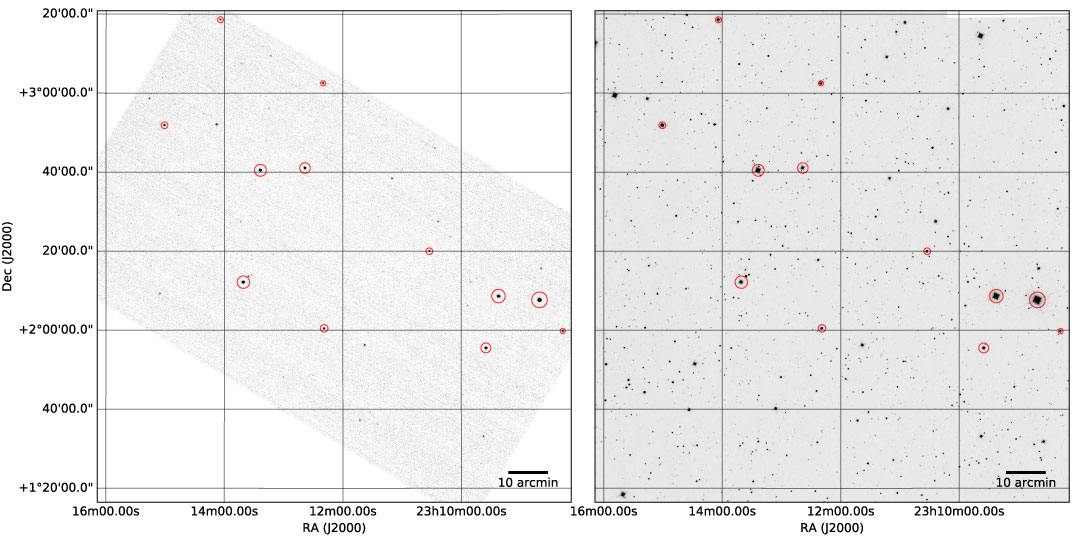
\includegraphics[width=1.5\textwidth]{Figures/starcam_images.jpg}
	\caption[Star camera example WISE]{\textit{Left}: Example of a background-subtracted star camera image with identified $>5\sigma$ sources circled in red. The orientation of the image on the celestial sphere is the one provided by BETTII's embedded star camera solver. This image corresponds to a field in the Scorpius constellation. \textit{Right}: WISE \SI{3.4}{\um} mosaic from the online archive, centered on the same location. This image is composed of 9 individual WISE images that we patched into a mosaic using the \textit{Montage}[CITE] software package.}
	\label{fig:starcamexample}
    \end{figure}
\end{landscape}
%\begin{landscape}
%\begin{figure}[!ht]
%	\centering
%	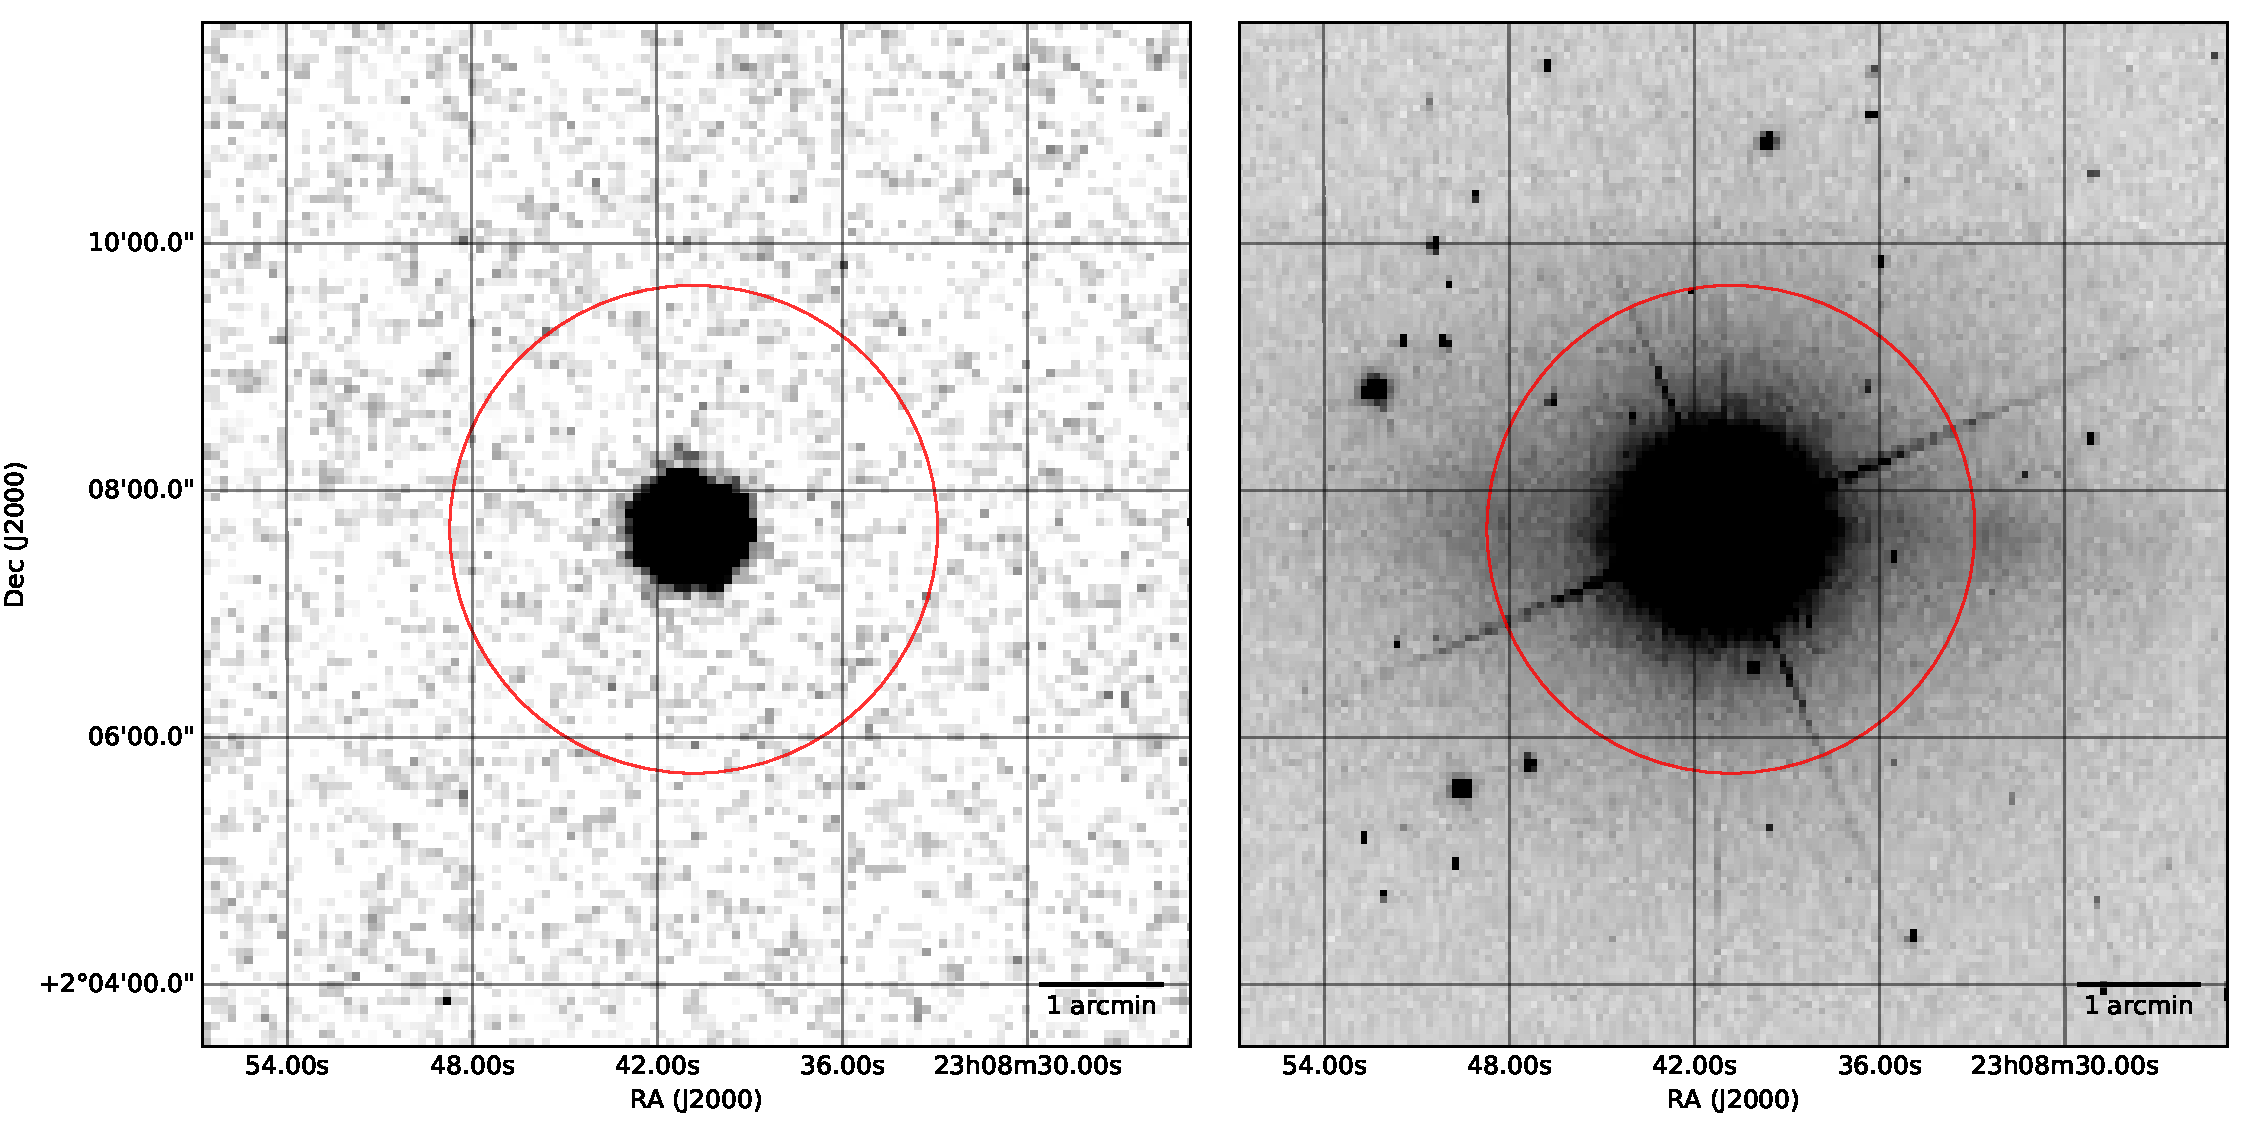
\includegraphics[width=1.5\textwidth]{Figures/starcam_SDSSr_zoom.pdf}
%	\caption[Star camera individual star]{\textit{Left}: Snapshot of a bright star seen within the background-subtracted star camera frame. \textit{Right}: Snapshot taken at the same location from the WISE \SI{3.4}{\um} archive.}
%	\label{fig:starcamzoom}
%    \end{figure}
%\end{landscape}

\subsubsection{Live star camera diagnostic software}

During our test operations, a lot of information is available and  it can sometimes be challenging to understand the full system status and diagnose the issues. To help mitigate this, we created a suite of small Python routines which help quickly diagnose the star camera behavior. For example, one software displays the latest image from the star camera, and overlays the blobs that the star finder software finds. At a glance, this can tell us if blobs are finding visible stars in the image, or if the star camera appears our of focus, or if there is a cloud cover. During flight, however, we will not have access to all this information because of the slow bandwidth. Hence, the software also cuts the star camera image (a $1920\times 1200$ array of 16-bit integers) into a smaller mosaic composed only of the regions around the blobs the software identified. Further, the type of all blobs is reduced to 8 bits. This constructs a much more modestly-sized piece of information that can be sent down for diagnostics.

Other metrics are useful to understand the star camera's behavior. For example, the star finder and catalog matching software solves for the best fit of exposure time, by comparing the known brightness of the stars and the measured number of digital counts on the detector. We find that this is accurate to $\sim 10-20\%$ in a vast majority of the cases, and values that are wildly off this estimate usually indicate either a false positive or some other sort of issue associated with the solving. This is used in two ways: first, it offers a quick sanity check that the solving happens correctly and robustly; and second, it can offer one additional protect against false position information, which we can use in the Kalman estimator when we decide to incorporate a star camera solution or not.


\section{Estimator implementation}

\subsection{Test setup and limitations}

The testing is done indoors in the Building 20 Highbay at NASA GSFC. The payload is sufficiently close to the rolling doors that one arm can see a small patch of sky while hanging from the indoor crane.

The payload is entirely run with 7 Marine Deep Cycle batteries, which provide all the required power for $\ge$\SI{8}{\hour} of continuous operations. BETTII is entirely wireless and uses a Wi-Fi router on board to provide high-bandwidth communication through a TCP/IP connection, which is useful for testing and displaying large quantities of information.

The mechanical, electrical, and communication setup is different than it will be in flight in several ways. First, the crane is about three times less high than the balloon train will be, which results in higher pendulum frequencies. Second, the payload can only see one arm at a time through the high bay doors, making it difficult to test the entire control system with the fine guidance sensor loop. Third, when the rolling doors are open, gusts of winds can move the payload as it is hanging, resulting in considerably larger pendulum motions than expected in flight. And finally, in flight, the communication bandwidth is expected to be 1~MB/s down and $\sim$1~B/s up. The astonishingly low uplink rate forces a minimalistic approach where most commands are only one or two bytes long. 

The star camera is also not put in its final, flight mounting position. The reason for this is that if the payload is lifted enough to clear most non-movable obstacles in the high bay, the angle at which the star camera can look and still see a patch of sky has to be less than $\sim \SI{30}{\degree}$. In previous months, star camera testing was done with the star camera positioned at the very end of one of BETTII's arms to increase the amount of sky coverage available. While discussions are underway to modify the high bay structure and open up portions of the wall, it is not reasonable to expect any actual changes for any of our relevant timescales for BETTII.


\subsection{Autofocus implementation}

Since the payload is close to the high bay door, changes in temperature occur and slightly change the focus of the star camera. These changes are expected to be more dramatic at float. For this reason, we implemented a very simple, yet very robust autofocus mechanism that we tested both on the ground and while hanging.

The algorithm relies on the fact that the focus ring of the lens has a hard stop. The stepper motor that controls the focus ring through a belt cannot pass this stop, and when it tries, the belt always slips. In addition, we also know that the focus position for the ring will always be very close to this hard stop, which is a little past infinity focus for the lens. 

Hence, we design an algorithm as follows:
\begin{enumerate}
\item Drive the stepper a large number of steps to guarantee hitting the hard stop.
\item Take a picture and move one step backward (away from the stop).
\item Calculate the variance of all the pixels in the image (which is a measure of sharpness).
\item Repeat a sufficient amount of times to guarantee passing through focus.
\item When done, go back to the position which maximized the variance.
\end{enumerate}

This very simple algorithm proved to be very robust in all situations. The variance metric was the simplest to implement, as opposed to more complicated sharpness metrics used in modern photography. We inspected the results by eye and they were always satisfactory. The small backlash usually present when the stepper motor changes direction to go to the best position is not noticeable in the results.

\subsection{Gyro attitude estimator}

We present here the results of the on-board Kalman filter estimator which was described in Chapter~\ref{chap:controls}. The data gathered through the many test runs is archived on the ground computer. We developed a framework in Python to process this data and align all quantities properly to BETTII's heartbeat. 

For this section, the results shown correspond to data gathered when the payload was sitting on the ground. This served as the simplest possible test to ensure the Kalman filter could appropriately correct for the errors given by the star camera. 

In Fig.~\ref{fig:GyroAttitudeEstimate}, we show the standard attitude plot. The red line indicates the inertial RA and DEC of the gondola or gyro reference frame estimated by the Kalman filter, while the blue dots indicates the measured inertial attitude of the same reference frame. In this plot, time goes from left to right (increasing RA). For each star camera data point, a line is drawn to show which estimator data point it corresponds to. This is necessary since the star camera solution is delayed with respect to the estimation. While the estimation starts as soon as the flight computer boots up, the first star camera solution resets it and sets a new starting point for the estimate.

\begin{figure}[!ht]
\begin{center}
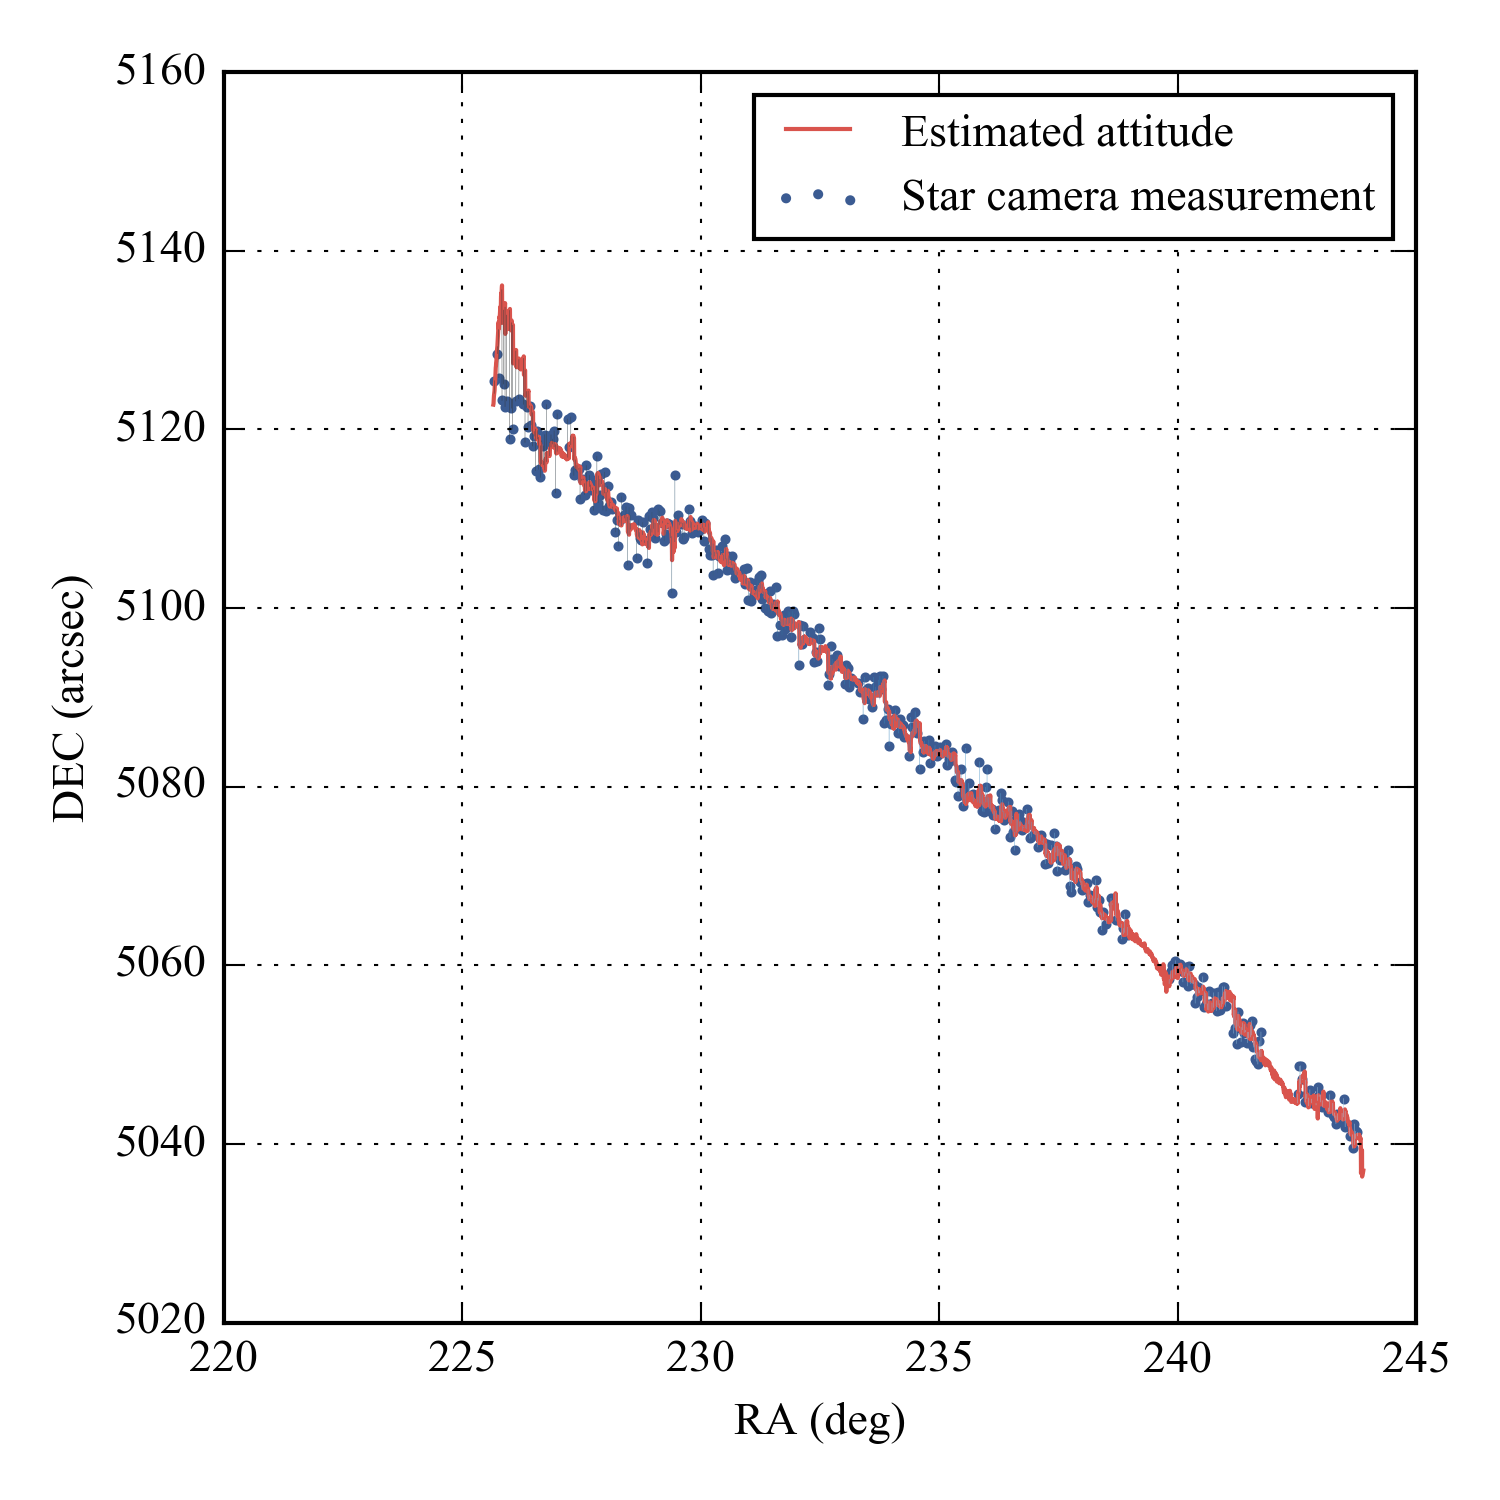
\includegraphics{Figures/attitude_estimate.png}
\caption[Attitude estimation while on the ground]{Attitude estimation while on the ground (see text for description).}
\label{fig:GyroAttitudeEstimate}
\end{center}
\end{figure}

In order to understand this plot in more details, we show two zoomed-in plots in Fig.~\ref{fig:AttitudeEstimateZoom}. The plot in (\subref{subfig:attitudeEstimateZoom1}) shows the beginning of the estimation process. At first, the star camera solutions appear systematically off from the estimates obtained from simply propagating the gyroscopes. Each time this happens, the Kalman filter adapts the bias to attempt minimizing this difference. After about $\sim 20$ solutions, it appears that the filter has converged to a mean deviation around zero. In (\subref{subfig:attitudeEstimateZoom2}), we show a zoomed-in snapshot towards the end of the run, where for some amount of time, no star camera solution was found - but given the slow drift of the gyroscopes, it is not too much of a problem and the solution found after some time is still very close to the estimate.

\begin{figure}[!h]
\begin{subfigure}[b]{0.5\textwidth}
		\centering
		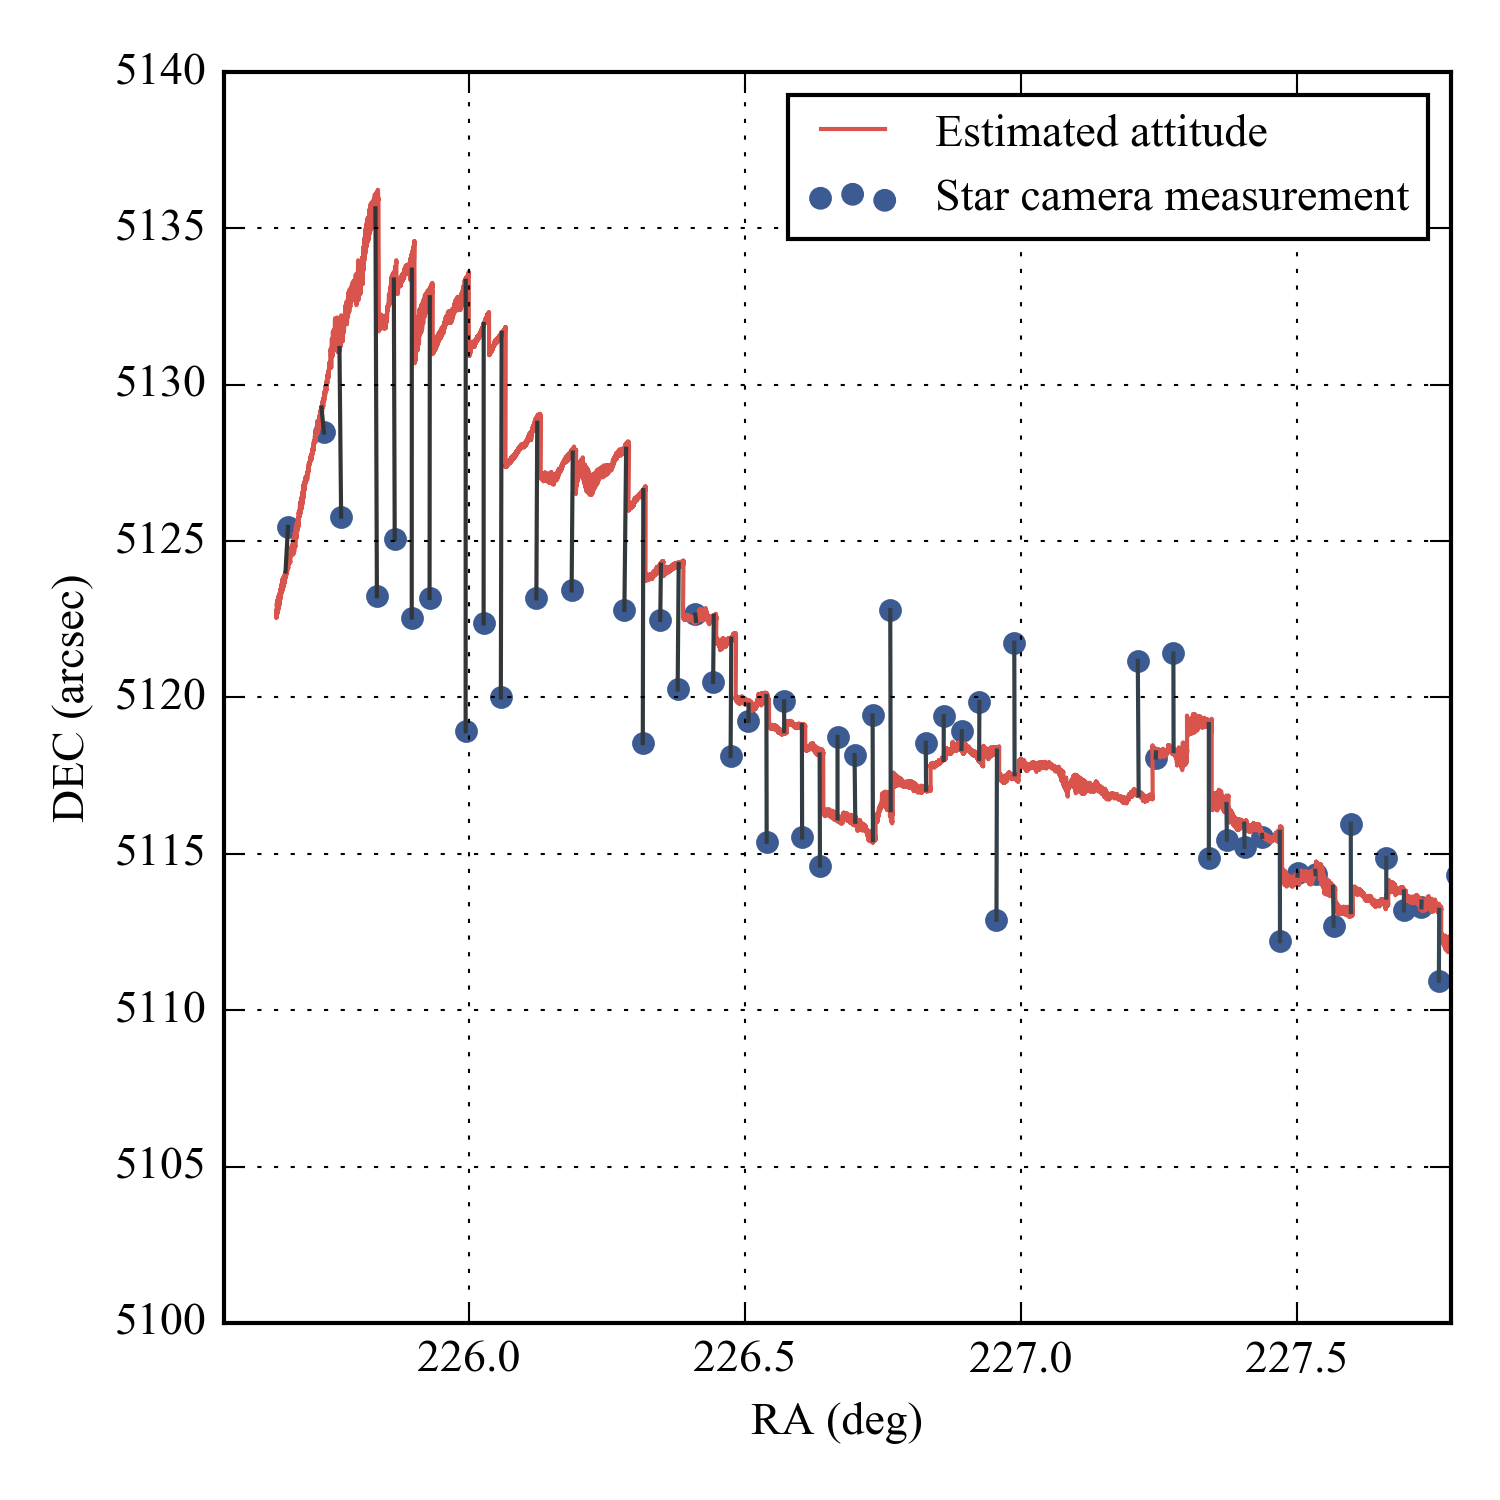
\includegraphics[width=0.98\textwidth]{Figures/attitude_estimate_zoom1.png} 
		\caption{}
		\label{subfig:attitudeEstimateZoom1}
\end{subfigure}
\begin{subfigure}[b]{0.5\textwidth}
		\centering
		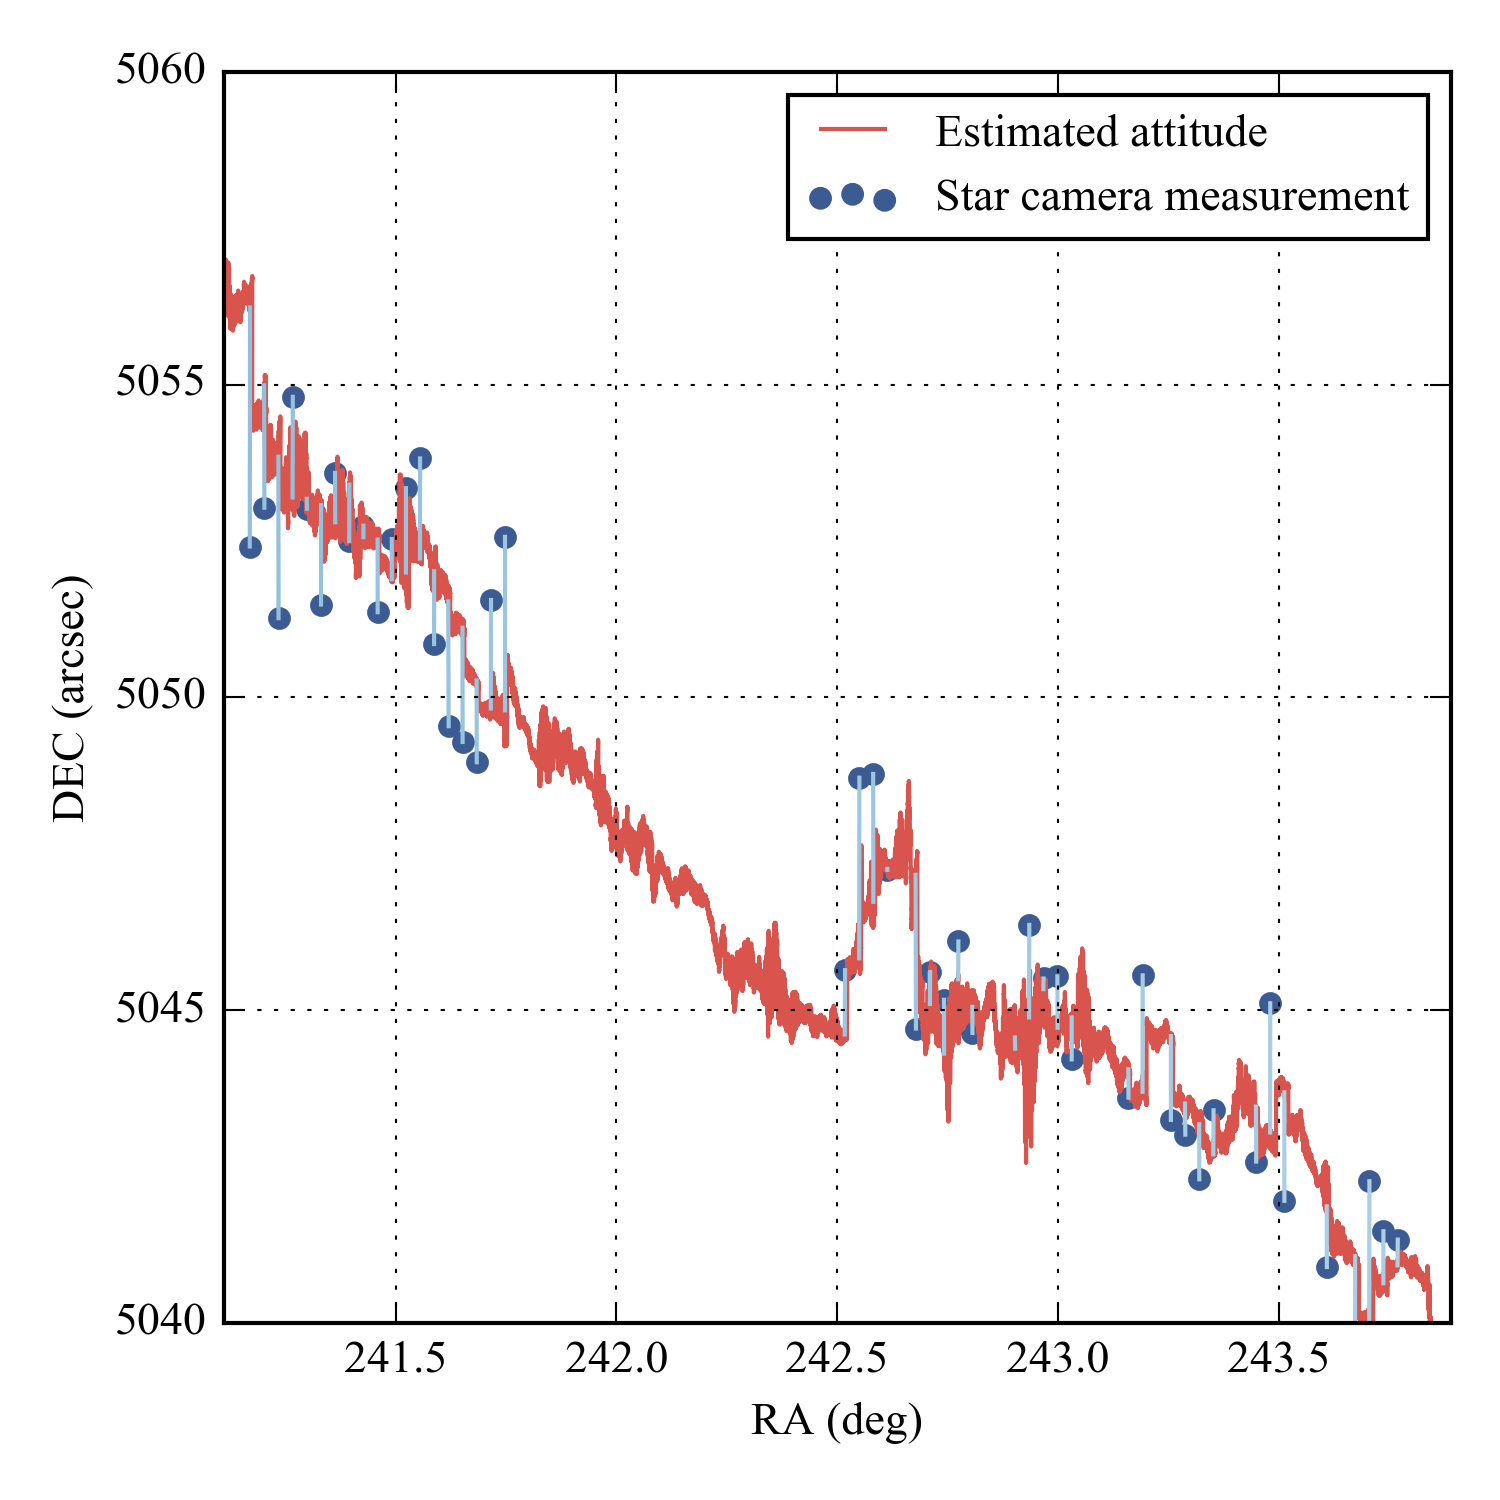
\includegraphics[width=0.98\textwidth]{Figures/attitude_estimate_zoom2.png} 
		\caption{}
		\label{subfig:attitudeEstimateZoom2}
\end{subfigure}
\caption[Zoom on attitude estimate plot]{Zoom on attitude estimate plot (see text for description).}
\label{fig:AttitudeEstimateZoom}
\end{figure}

For each star camera solution, the software estimates a correction to apply to the bias that modifies the perceived gyro velocity. The results of this bias estimation for this particular run are shown in Fig.~\ref{fig:BiasEstimate}. Note that since the star camera is inherently less sensitive in roll (about X), the X bias estimate is more noisy and takes longer to converge. 
\begin{figure}[!h]
\begin{center}
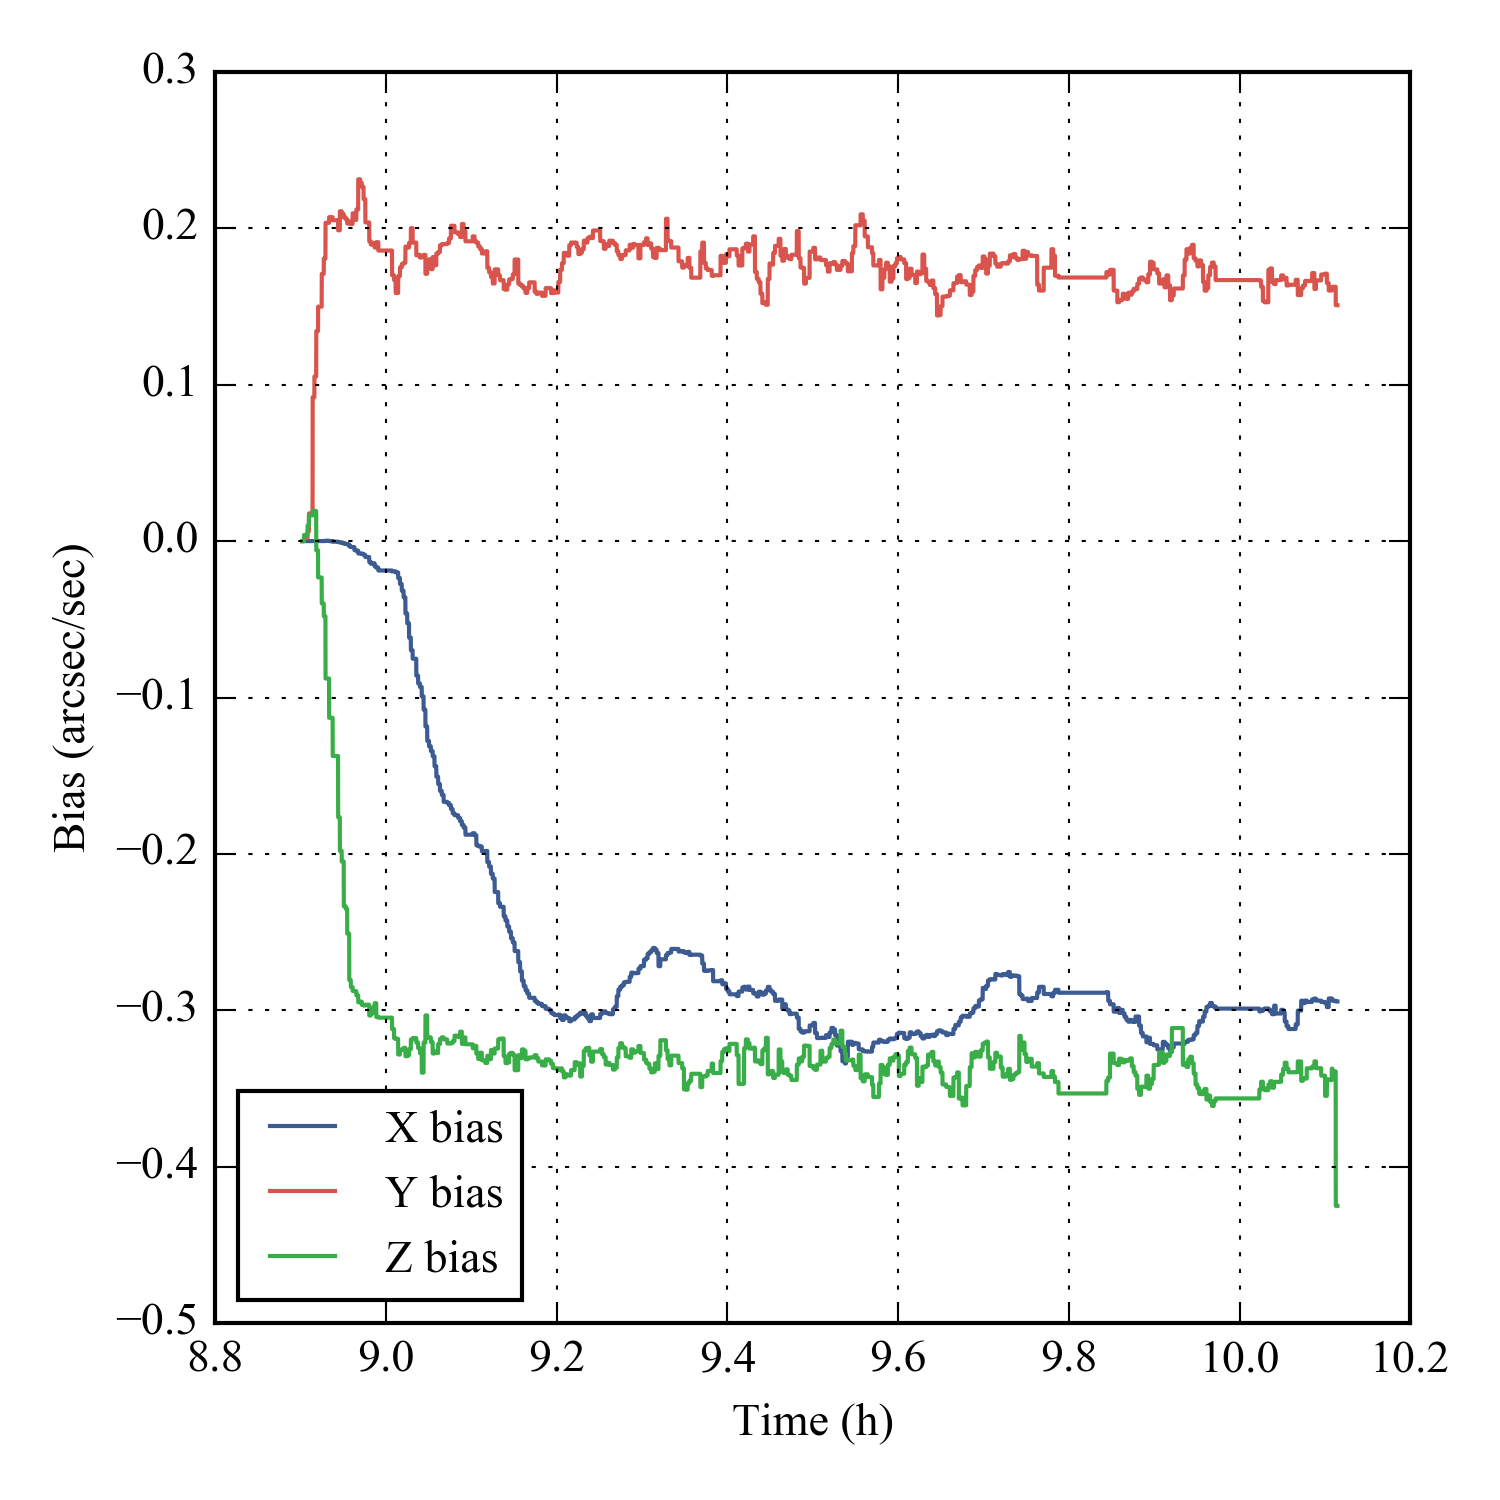
\includegraphics[width=0.7\textwidth]{Figures/bias_estimate.png}
\caption[Bias estimation while on the ground]{Bias estimation while on the ground.}
\label{fig:BiasEstimate}
\end{center}
\end{figure}

Finally, we can display the error between the estimated and measured attitude in a single scatter plot (Fig.~\ref{fig:MeasuredVsEstimated}). The contours show a 2D Kernel density estimation on the dataset, indicative of how peaked the probability distribution is. For this particular run and including the Kalman filter learning process at the beginning, we obtain an overall standard deviation of \ang{;;2.3}. Note that the peak of the distribution is not exactly located at (0, 0), which indicates an error in the alignment of the star camera solution with the corresponding estimator loop number. This is a known mistake from the processing software that was corrected since then.

\begin{figure}[!h]
\begin{center}
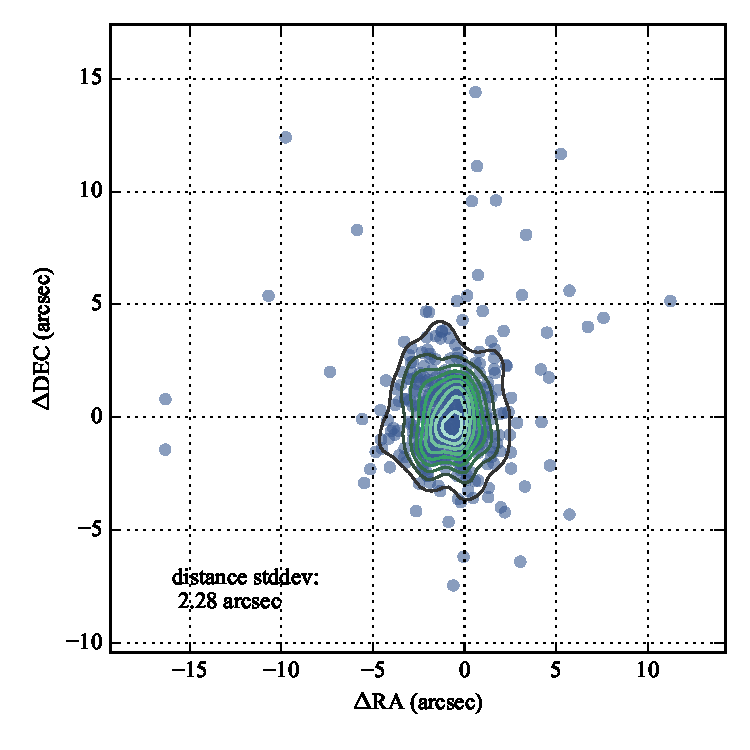
\includegraphics[width=0.7\textwidth]{Figures/measured_vs_estimated.pdf}
\caption[Error between measured position and estimated position]{Error between measured position and estimated position.}
\label{fig:MeasuredVsEstimated}
\end{center}
\end{figure}




%\subsubsection{Testing the Kalman filter software with simulated data}
%\subsubsection{Test results when sitting on the ground}
\subsection{Telescope attitude estimator}

While knowing how the gyroscope gondola is oriented is critical to properly command the actuators (which are in that reference frame), the real error perceived by the instrument and the optics is the error in the telescope reference frame. The figure we used in the previous chapter is put here again for convenience and to set the context of the relevant reference frames (Fig.~\ref{fig:starcamRefFrame2}). What is not shown on this picture is the fact that the telescope reference frame itself is rotated about $\vectors{y}_\tel$ by some elevation angle with respect to the gyro reference frame. 

\begin{figure}[!ht]
	\centering
	\includestandalone{Figures/starCameraRefFrame}
	\caption[The star camera reference frame]{See text for details.}
	\label{fig:starcamRefFrame2}
  \end{figure}

The error vector is estimated in the local telescope reference frame by knowing the inertial attitude of the telescope, which is related to the inertial attitude of the star camera and the gyro reference frame. The target's coordinates can then be determined in the telescope reference frame, since we know the target's inertial coordinates. The two spherical angles that we obtain are $\Delta\crossEl$ and $\Delta\El$, which are the cross-elevation and the elevation angles, respectively. 


\subsection{Phase estimator}

The phase estimator is perhaps the most constraining aspect of this mission. Indeed, in order to properly reconstruct interferograms, the phase uncertainty needs to be extremely small, which leads to a desired attitude uncertainty the order of $\sim$\ang{;;0.1} for periods of minutes. This quantity is exclusively in cross-elevation, as elevation errors do not contribute any pathlength error. 

The various components that create delay are summarized here. By far the largest delay errors will be introduced by attitude pointing errors, which correspond to the errors in cross-elevation. These errors are corrected by the Warm Delay Line to some uncertainty. In addition to those errors, the Cold Delay Line is also adding some errors. Finally, there can remain errors introduced by thermal variations of the structure.

The zero-point adjustment of the delay can be done using fringe tracking in the science channels using a bright calibrator star (see Appendix~\ref{AppendixA}.\ref{apsec:fringeTracking}). This will allow to correct for errors that are large on longer timescales. Assuming that this scheme works (it can only be tested in flight), then the only errors that are present on short timescales are the errors from the two delay lines and the attitude motion. 

Without an absolute zero-point correction on shorter timescales, the phase estimator relies exclusively on our attitude estimator, which will consist of the bulk of the error. The phase or OPD estimate is then $\OPD = \crossEl\units{\si{\radian}}\times \SI{8}{\meter} $, which is then fed to the WDL for correction. For scaling, a \ang{;;1} attitude error corresponds to \SI{40}{\um} error of OPD. 

The tuning of the WDL and CDL was successfully achieved and is discussed elsewhere (Dhabal \textit{et al} 2016, in press).



\section{Pointing tests and performance results}

\subsection{Control system in practice}

In practice, there are only a few key knobs that are required to pilot BETTII to its inertial attitude. The most sensitive knobs are the PID gains for the azimuth loop and the momentum dump loop, as they drastically change the response of the payload. 

However, the Kalman filter also imposes more knobs, which have a more abstract role in the attitude estimation phase of the code. For our 6-state Kalman filter estimator, 9 knobs are nominally available. These knobs act as three sets of ($\vectors{x}, \vectors{y}, \vectors{z}$) weights to increase or decrease the relative importance of the measurements and process noise. The three sets control: the weight of the gyroscope measurements; the weight of the bias rate of change; and the weight of the star camera solution. These weights multiply the variance of the various contributors, and will influence the way the estimator treats each incoming piece of information. The software uses by default the theoretical values for the relative weights, computed in Section~\ref{sec:SensorModels} of the previous chapter, but allows the user to tweak those knobs. 

For example, increasing the weight of the bias indicates to the estimator that the bias is expected to vary more, allowing for faster convergence of the bias to its final solution, but with larger statistical variation in steady-state. On the contrary, a very small weight to the bias indicates that the bias is almost not expected to change, so the steady-state will have very little variation, but the impact of a new star camera measurement will be much decreased. 

The star camera uses weights that are directly measured by the solving software. When a catalog pattern match is found, a least-square estimate of the best position naturally leads to errors in RA, DEC, and ROLL. as shown in Table.~\ref{tab:starCameraTests}, the error in ROLL is considerably larger than the error in RA and DEC, so the ROLL component of the star camera solution should not be trusted as much as the other two components. 

One indirect impact of these weights is how much change is going to be induced each time a new measurement comes in. Fig.~\ref{fig:AttitudeEstimateZoom} shows distinct jumps in the gyroscope estimated position, which are caused by the fact that the camera is trusted perhaps too much. These jumps are getting smaller as the solution converges, but could still cause controls problems in the future, as they are injected directly in the determination of the errors in the PID controllers. Hence, the star camera gains should be small when the star camera first attempts to determine the bias steady-state values, but should be increased when tracking to avoid trusting new measurements too much and causing jumps in the control system. 

For flight, we plan to reduce these 9 Kalman filter knobs to only three (one per system, as opposed to one per axis for each system), hence simplifying the commanding from the ground. We have determined the validity of this approach in the lab.

\subsection{Gondola pointing stability with high bay doors closed}

The most common test that we do routinely is to test the pointing stability indoors, without using the star camera. This corresponds to a pure controls test, since the star camera is not functional and we do not have knowledge of the real RA and DEC of the payload. 

When the payload is lifted and hangs uncontrolled, the motion about $\vectors{z}$ is shown in Fig.~\ref{fig:intgralgyroZ400}, and the power spectrum of the velocities is shown in Fig.~\ref{fig:multiPSD400_lifted}. The motion can be mostly characterized by an oscillation with a $\sim\SI{100}{\second}$ period, which likely is caused by the restoring torque from the crane's geometry. The excitation is likely caused by the A/C of the high bay room, as well as small motions of the high bay structure itself.

\begin{figure}[!ht]
\begin{center}
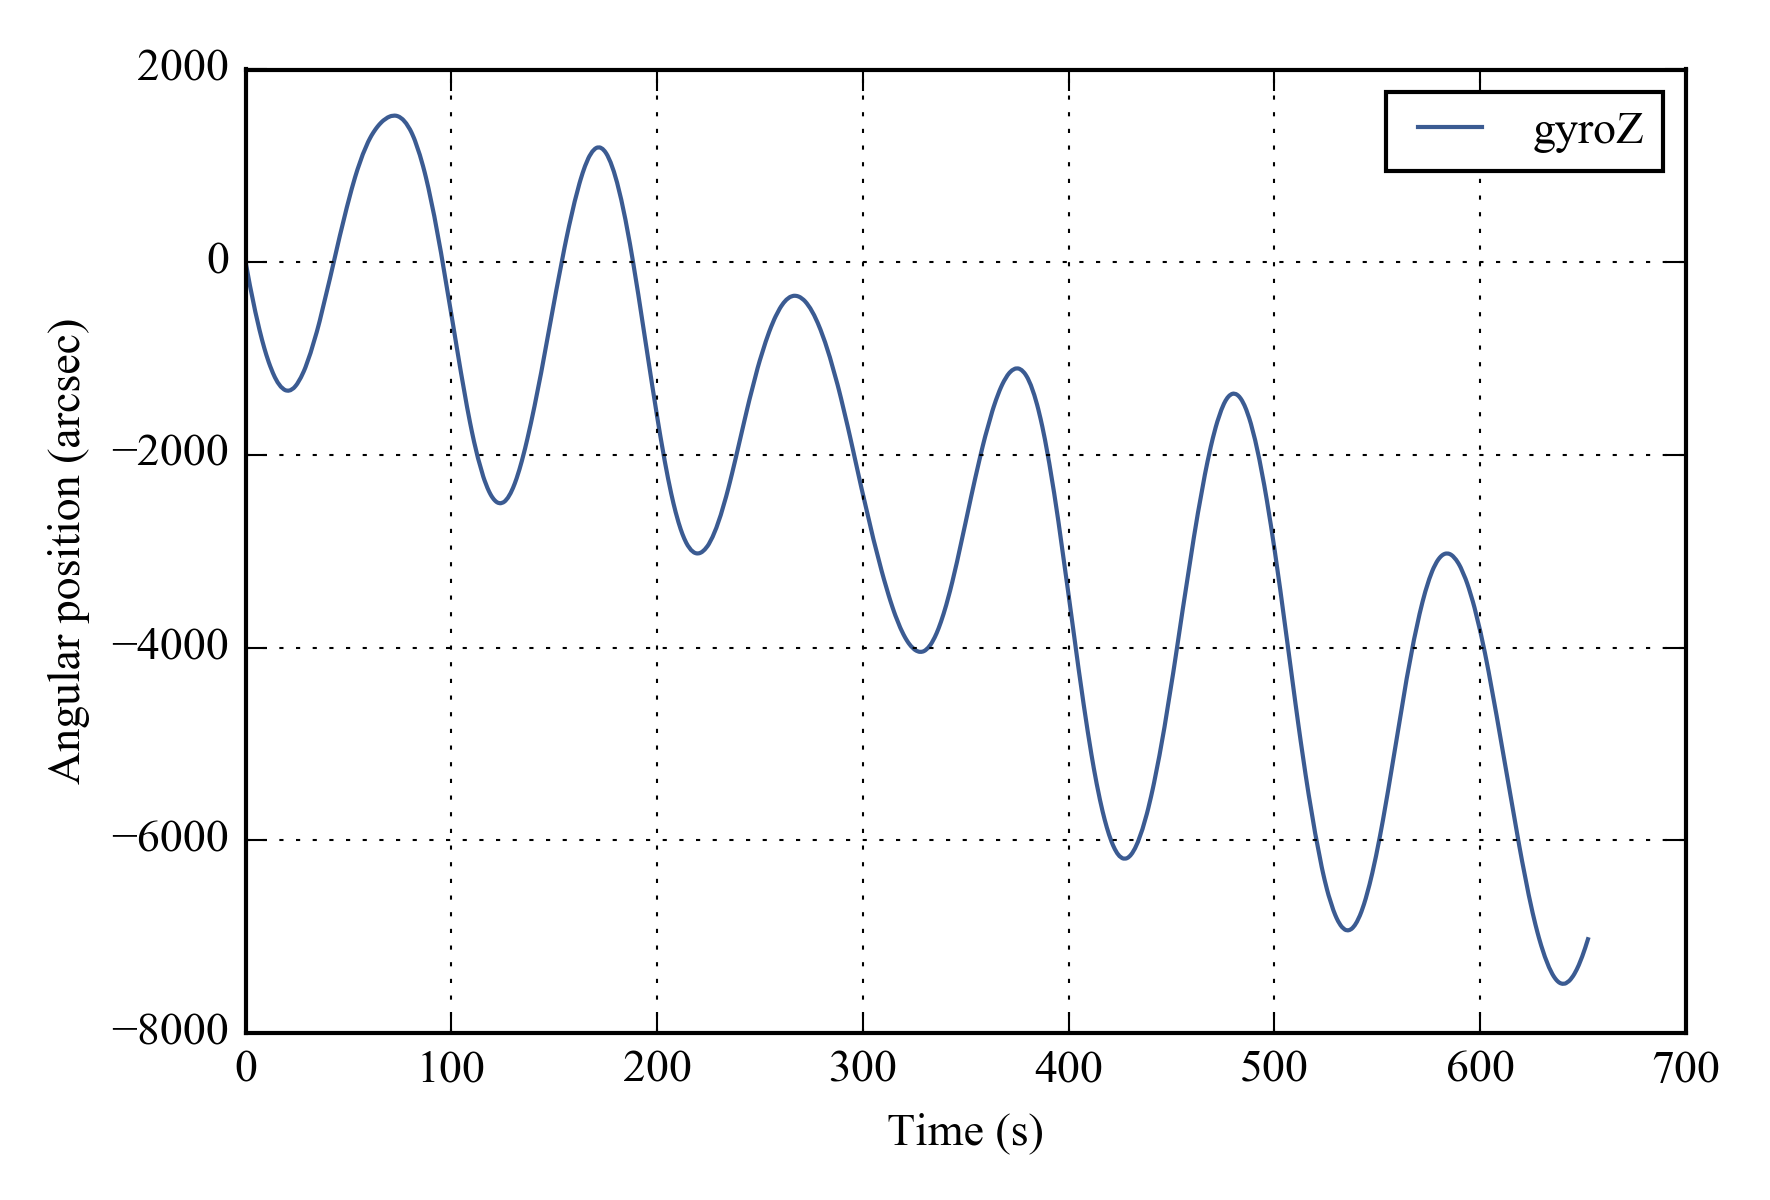
\includegraphics{Figures/integral_lifted_gyroZ.png}
\vspace{-0.5cm}
\caption[Integrated gyro time series while hanging]{Integrated gyro time series while hanging and no motor on.}
\label{fig:intgralgyroZ400}
\end{center}
\end{figure}

The PSD plots in Fig.~\ref{fig:multiPSD400_lifted} show that most of the motion occurs in $\vectors{z}$ at about \SI{0.01}{\hertz}. This motion is 3 orders of magnitude higher than any other contributor about $\vectors{z}$. We can also notice a peak at \SI{0.7}{\hertz} that is visible in all axes, which we believe is an uncontrolled pitch motion of the payload about its long axis. This can be caused for example by a pivot mode about the gondola attachment pin. Since we see the signature of this peak in all axes, this is further indication of the non-orthogonality of the gyroscope mount. The peak at \SI{0.5}{\hertz} is thought to be caused by a pivot mode about the same point but about the $\vectors{x}$ axis. The ratio of the two peak frequency roughly corresponds to the expected ratio of the moment of inertia about $\vectors{y}$ and $\vectors{x}$. The peak at \SI{0.15}{\hertz} seen in both $\vectors{x}$ and $\vectors{y}$ is attributed to the pendulum mode about the crane attachment on the rook. This is consistent with a pendulum frequency $\frac{1}{2\pi}\sqrt\frac{g}{L}$ for $L\sim\SI{20}{\meter}$. In flight, we expect that last mode to be at even lower frequency, by at least a factor of $\sqrt{5}$, as the balloon train is expected to be at least 5 times longer.

%\begin{figure}[!h]
%\begin{center}
%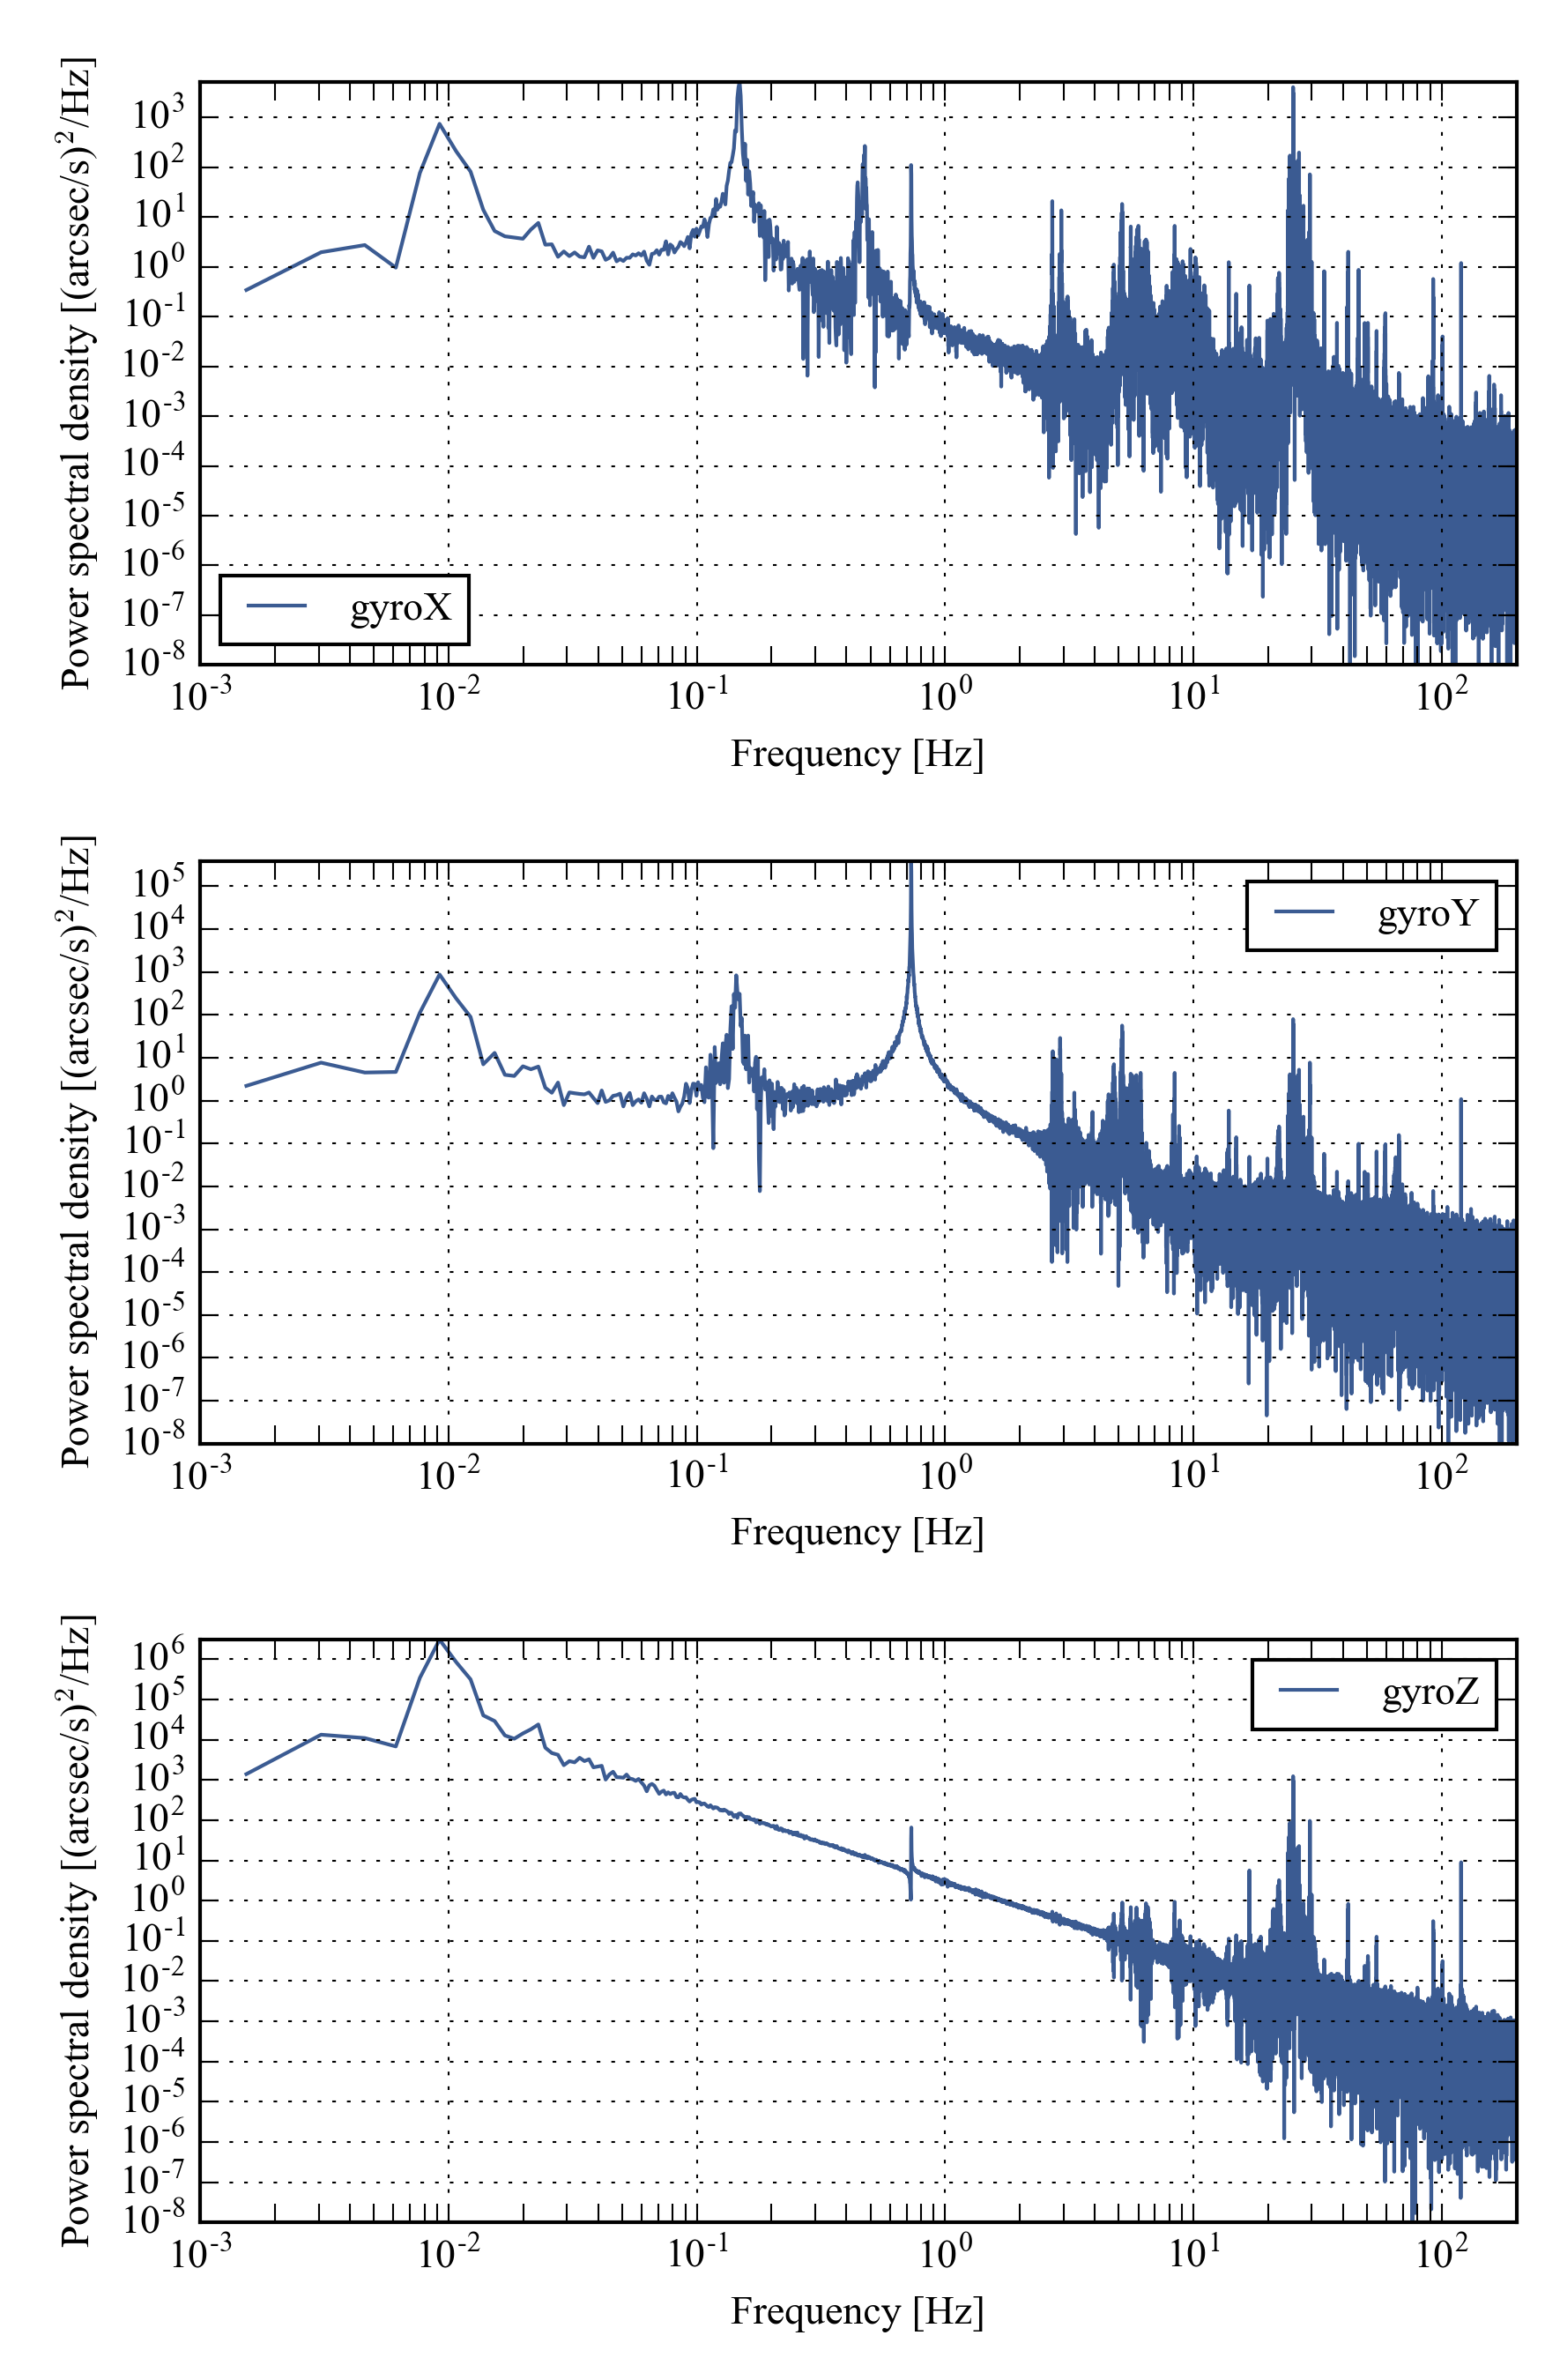
\includegraphics{Figures/lifted_400.png}
%\label{fig:multiPSD400_lifted}
%\vspace{-0.5cm}
%\caption[Gyro PSD with payload lifted]{Gyro PSD with payload lifted.}
%\end{center}
%\end{figure}

\begin{landscape}
\begin{figure}[!h]
\begin{subfigure}[b]{0.7\textwidth}
		\centering
		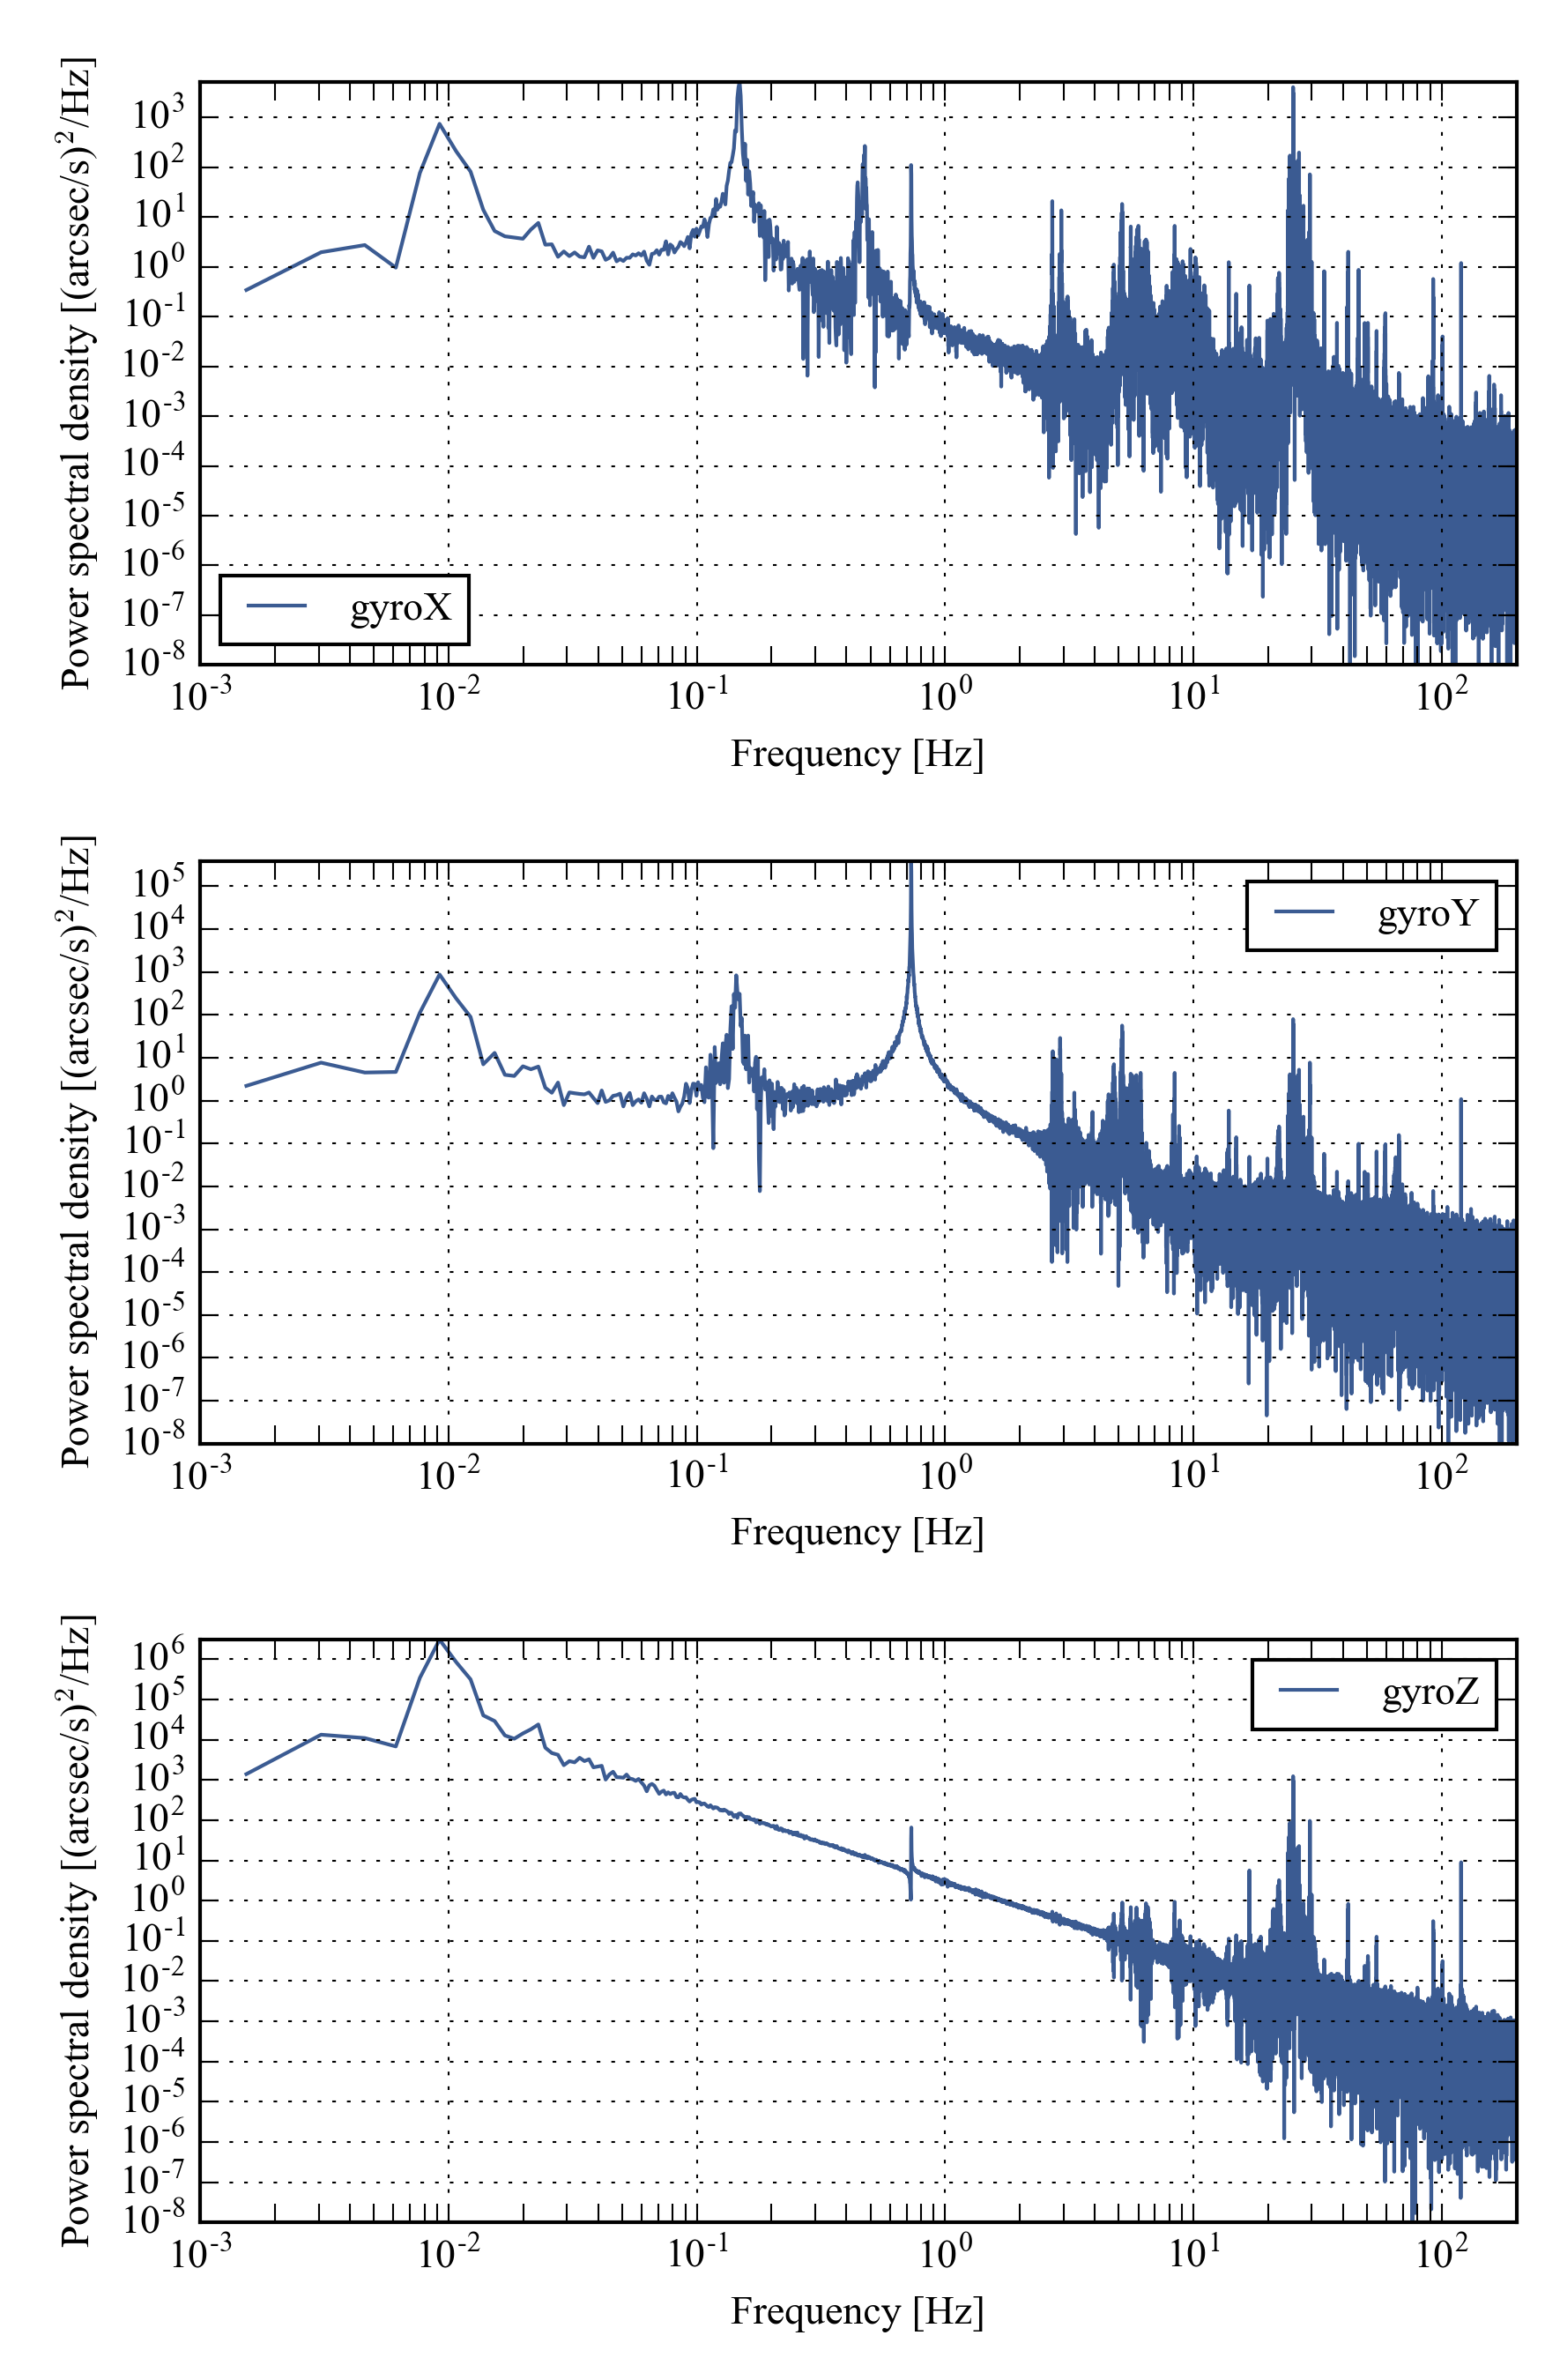
\includegraphics[width=0.98\textwidth]{Figures/lifted_400.png}
	\vspace{-0.5cm}
	\caption{}
	\label{fig:multiPSD400_lifted}
	\end{subfigure}
\begin{subfigure}[b]{0.7\textwidth}
		\centering
	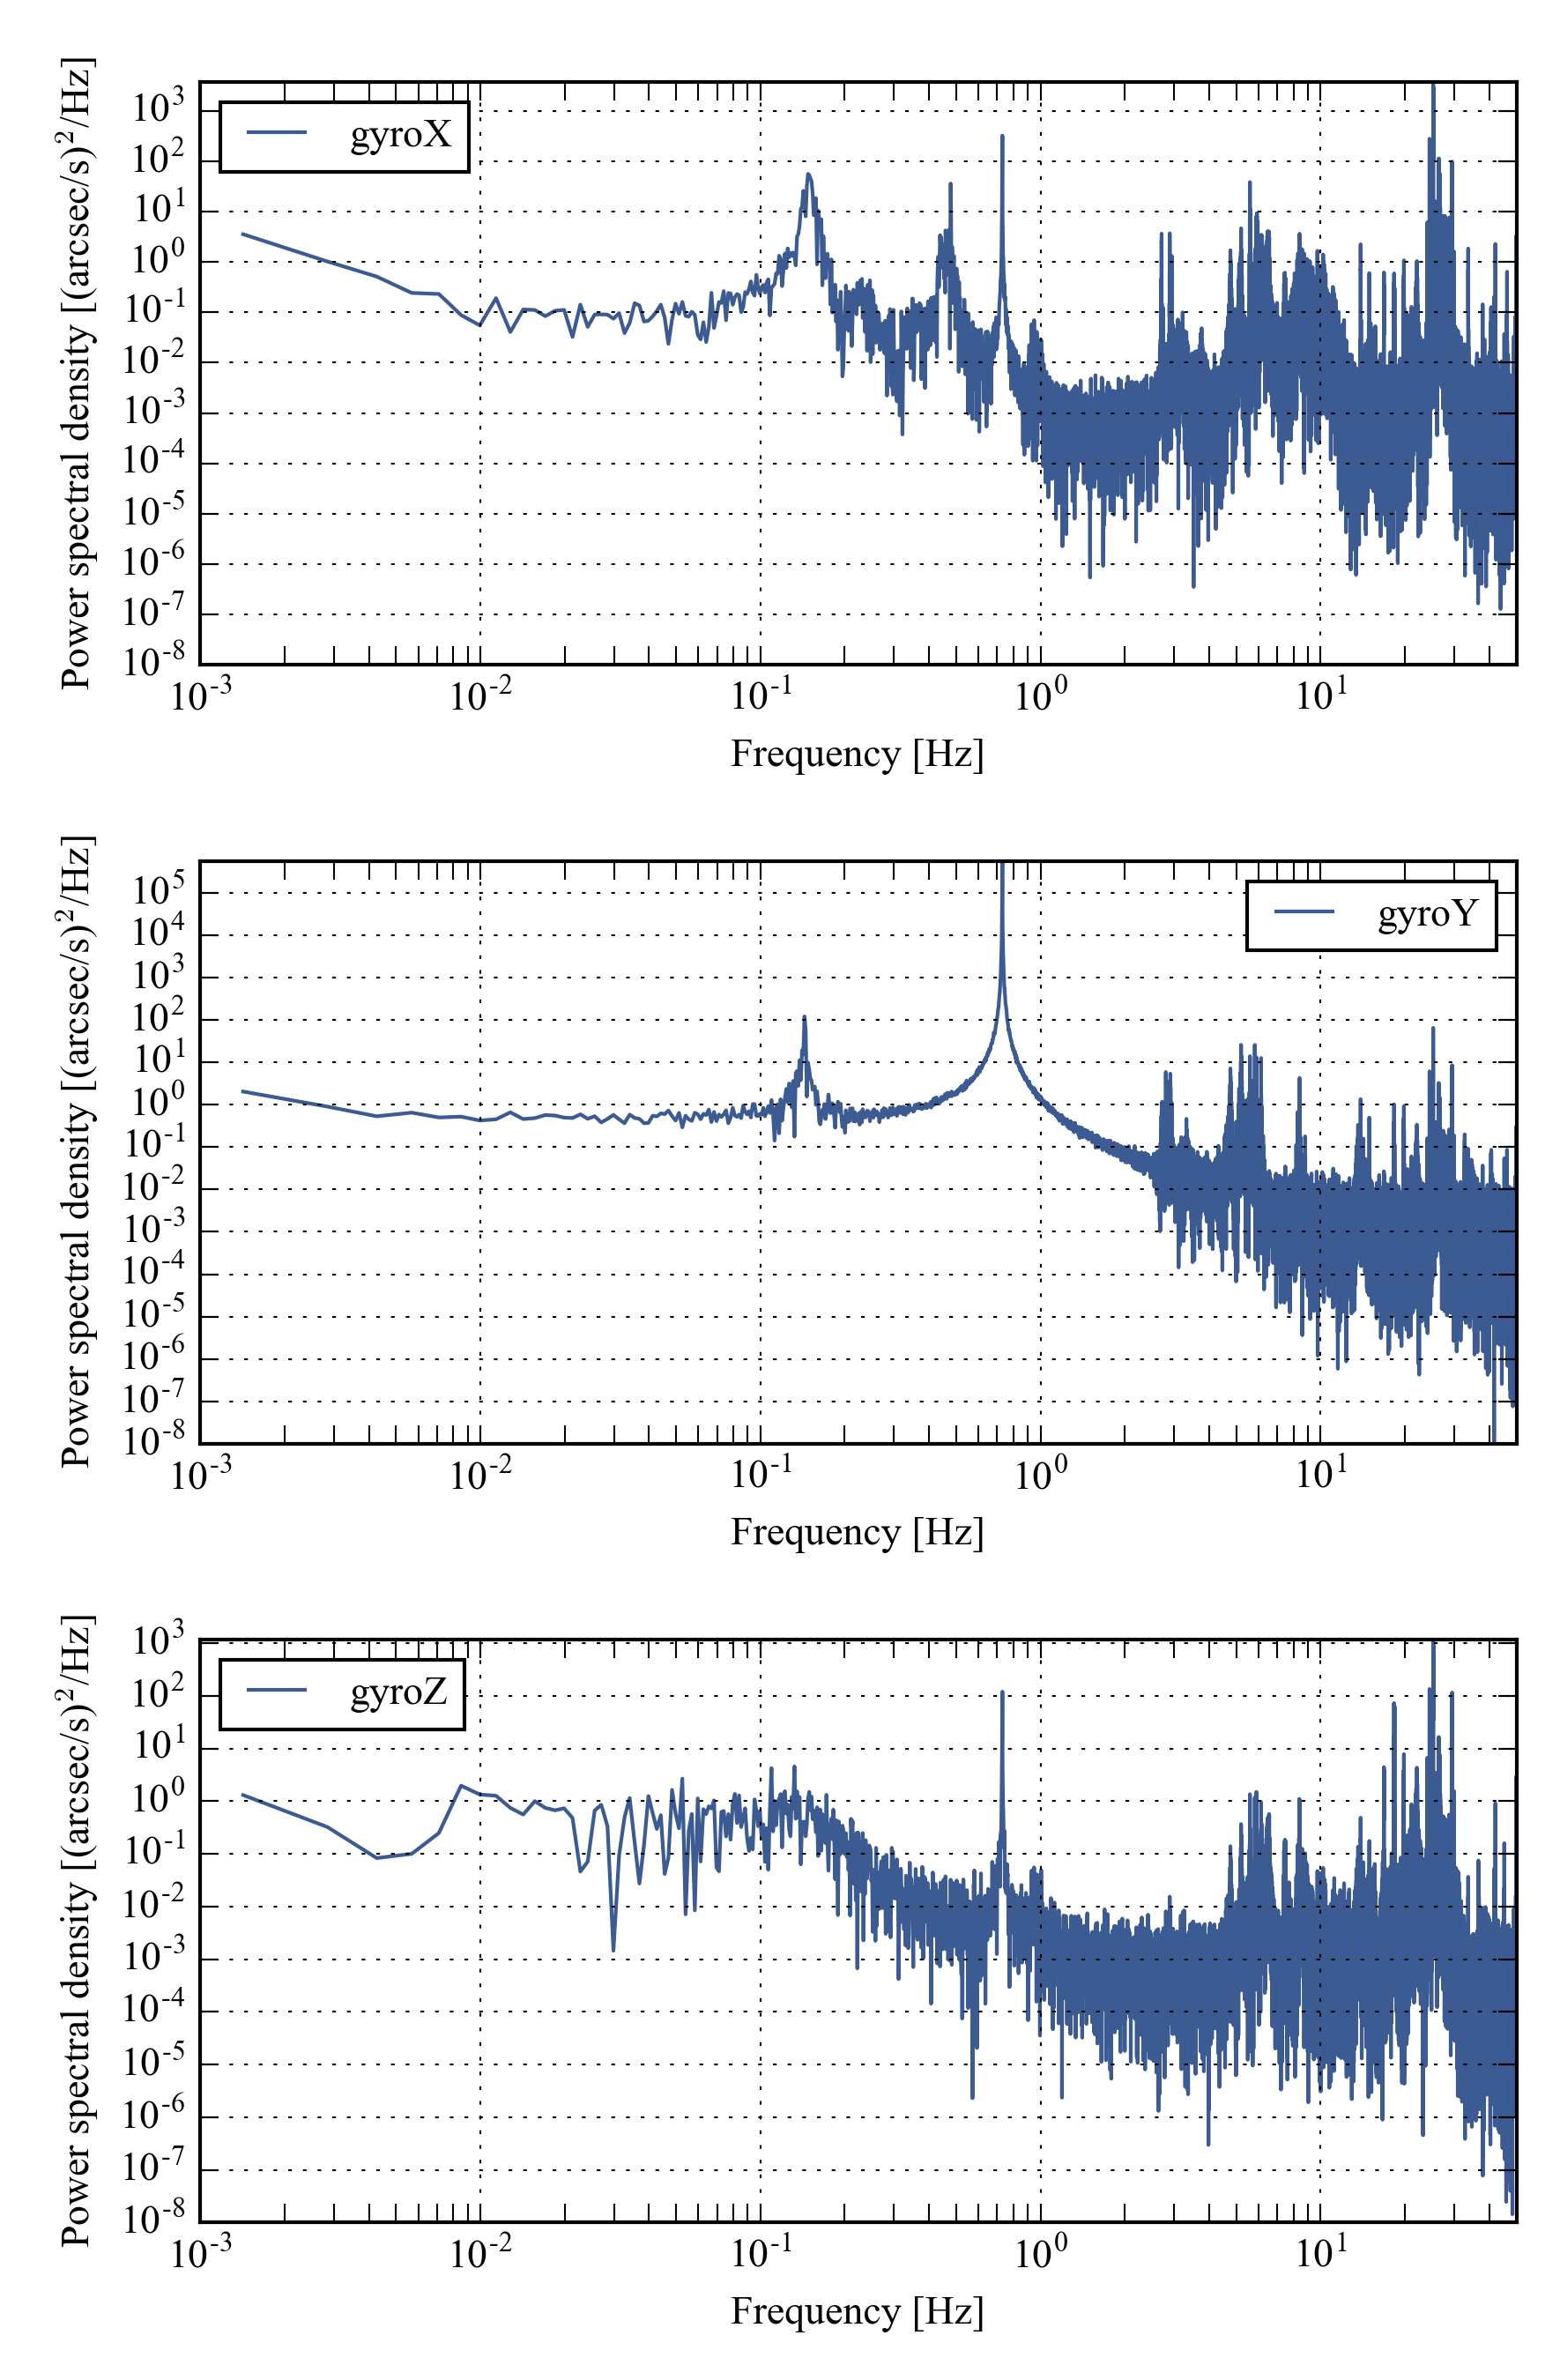
\includegraphics[width=0.98\textwidth]{Figures/multiPSD100.png}
	\caption{}
	\label{fig:multiPSD100_controlled}
	\end{subfigure}
\caption[Noise while hanging]{Noise while hanging indoors}
\label{fig:multiPSD}
\end{figure}
\end{landscape}



Once lifted, the gyro PSD about $\vectors{z}$ is quite different (see Fig.~\ref{fig:multiPSD100_controlled}). We are indeed able to cancel out most of the drift by about 6 orders of magnitude in power at \SI{0.01}{\hertz}. The resulting time series showing the cross-elevation angle is shown in Fig.~\ref{fig:simplePlot_crossEl}. The 1$\sigma$ r.m.s noise of this \SI{700}{\second} run is $\le\ang{;;1}$. This reflects a 1000:1 rejection ratio when the control loop is on.

%\begin{figure}[!h]
%\begin{center}
%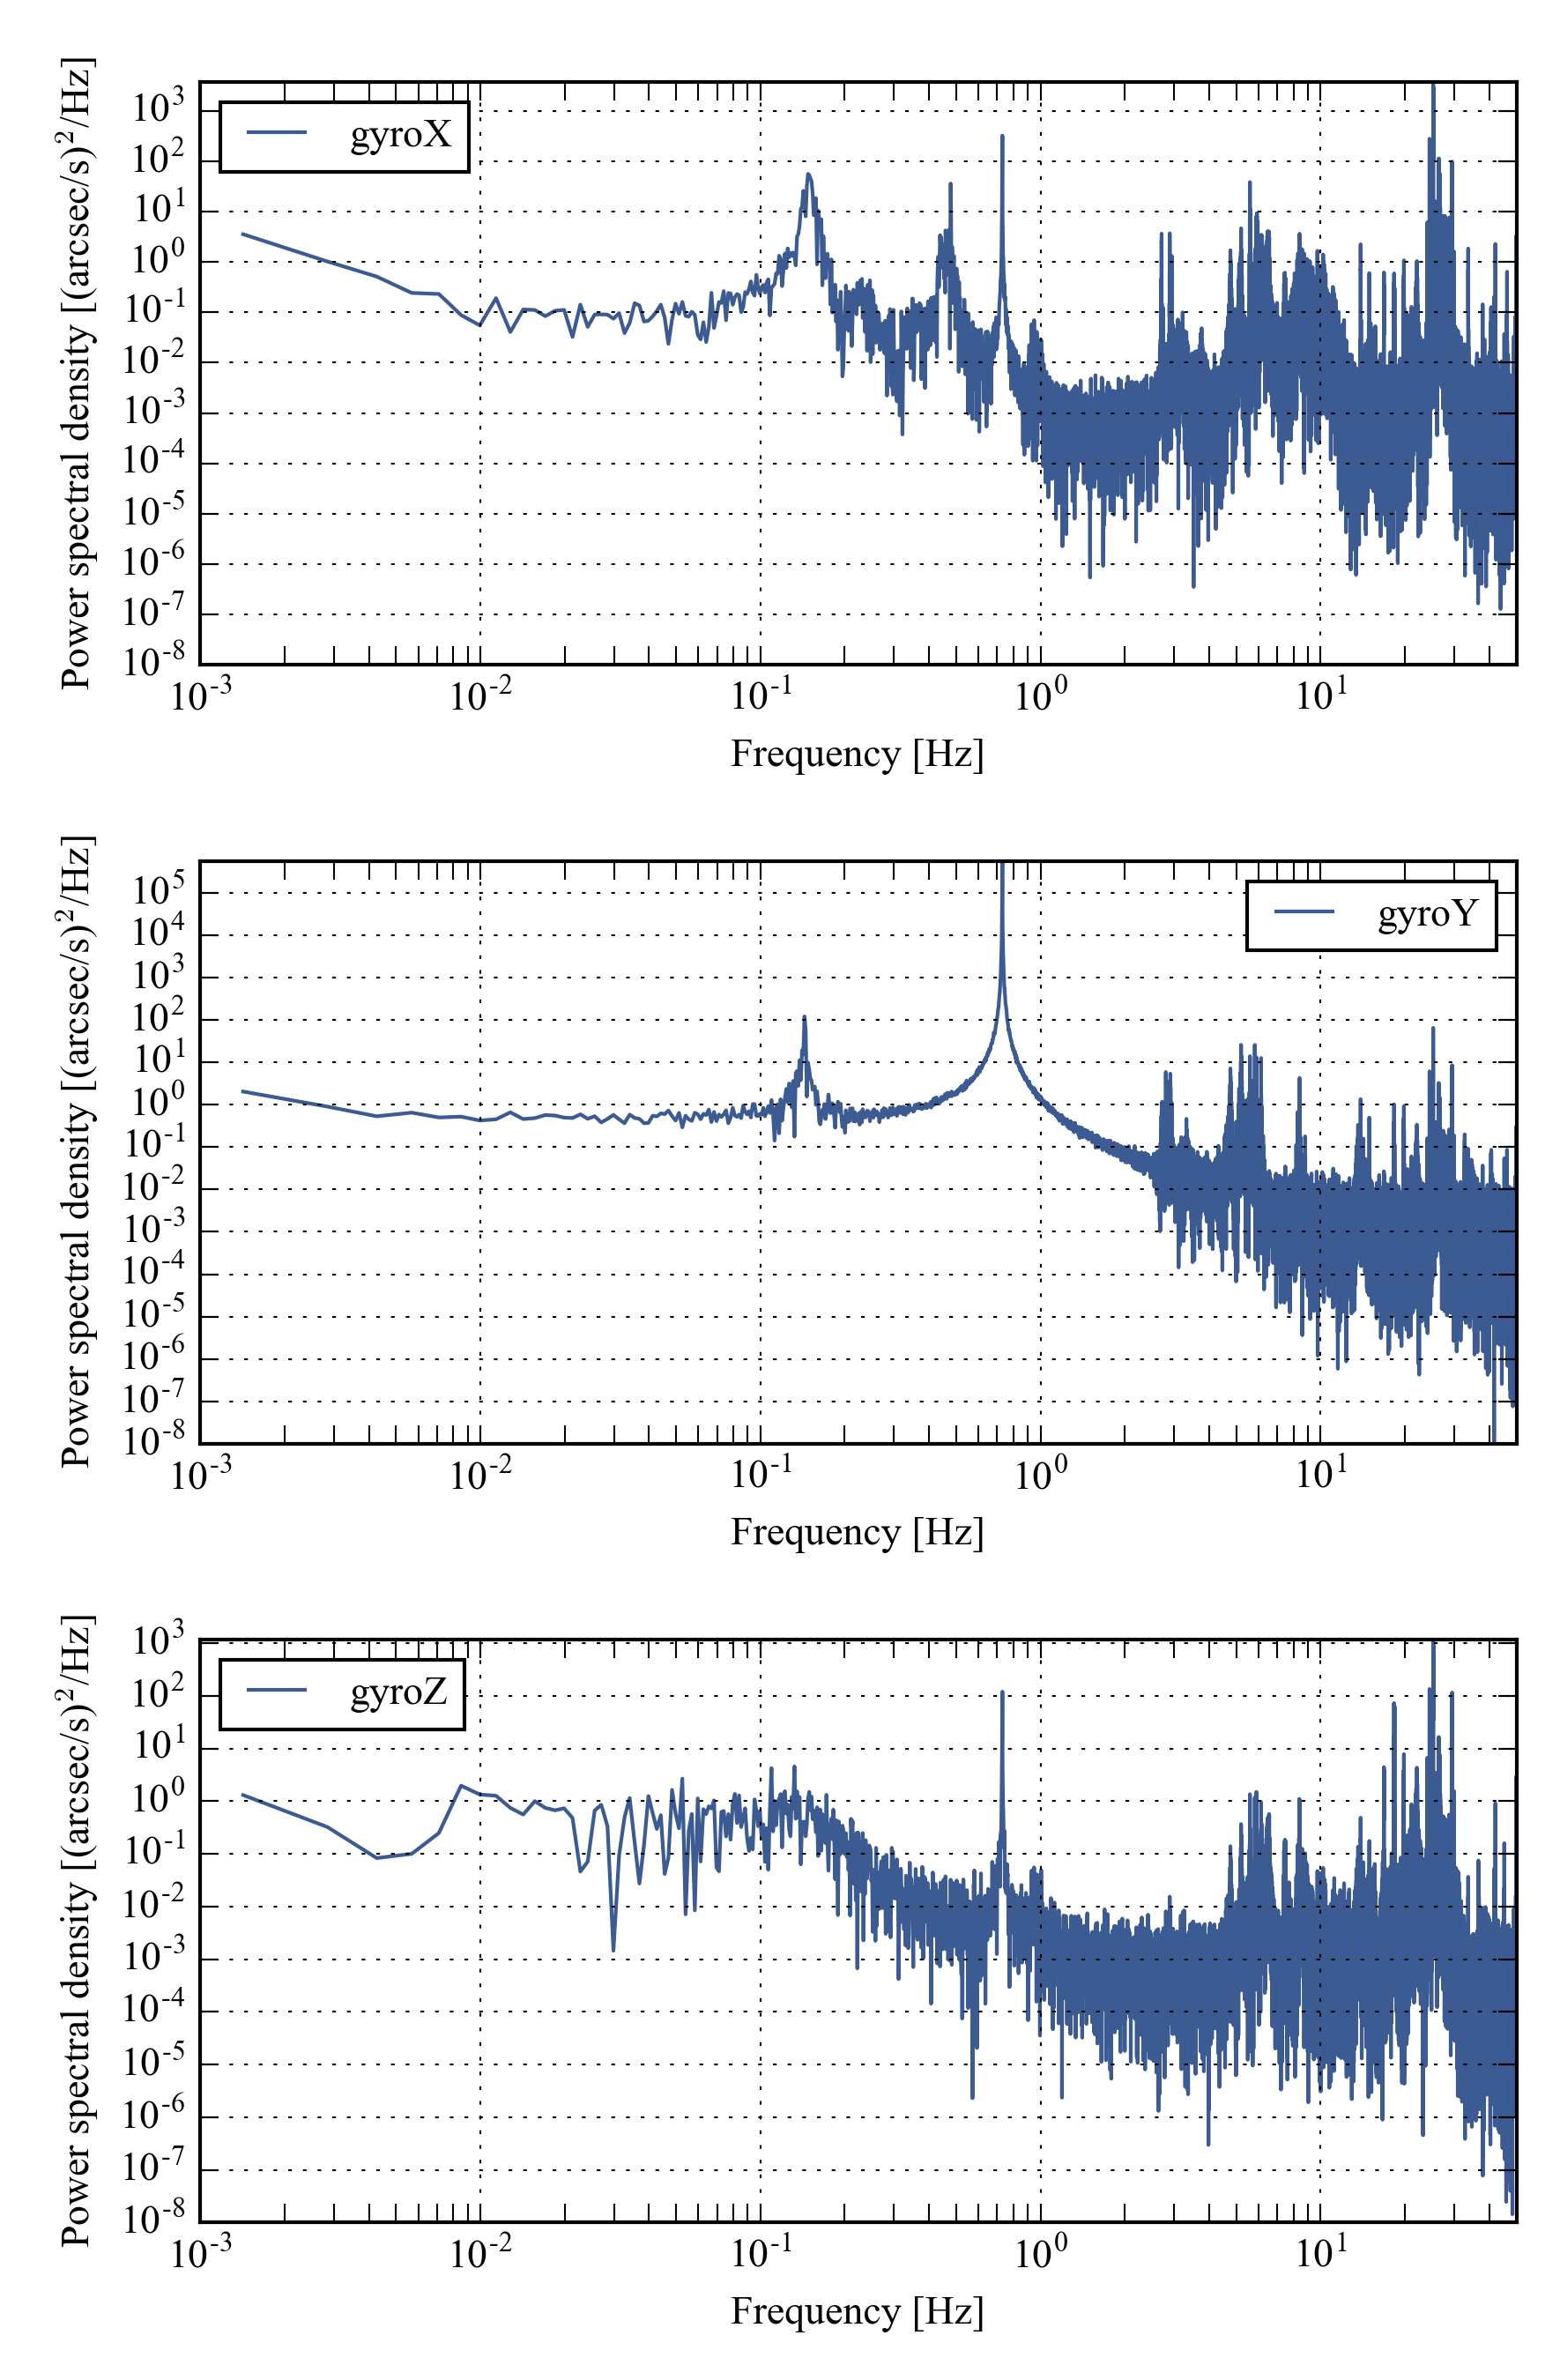
\includegraphics{Figures/multiPSD100.png}
%\label{fig:multiPSD100_controlled}
%\vspace{-0.5cm}
%\caption[Gyro PSD with payload lifted, under azimuth control]{Gyro PSD with payload under azimuth control.}
%\end{center}
%\end{figure}

\begin{figure}[!h]
\begin{center}
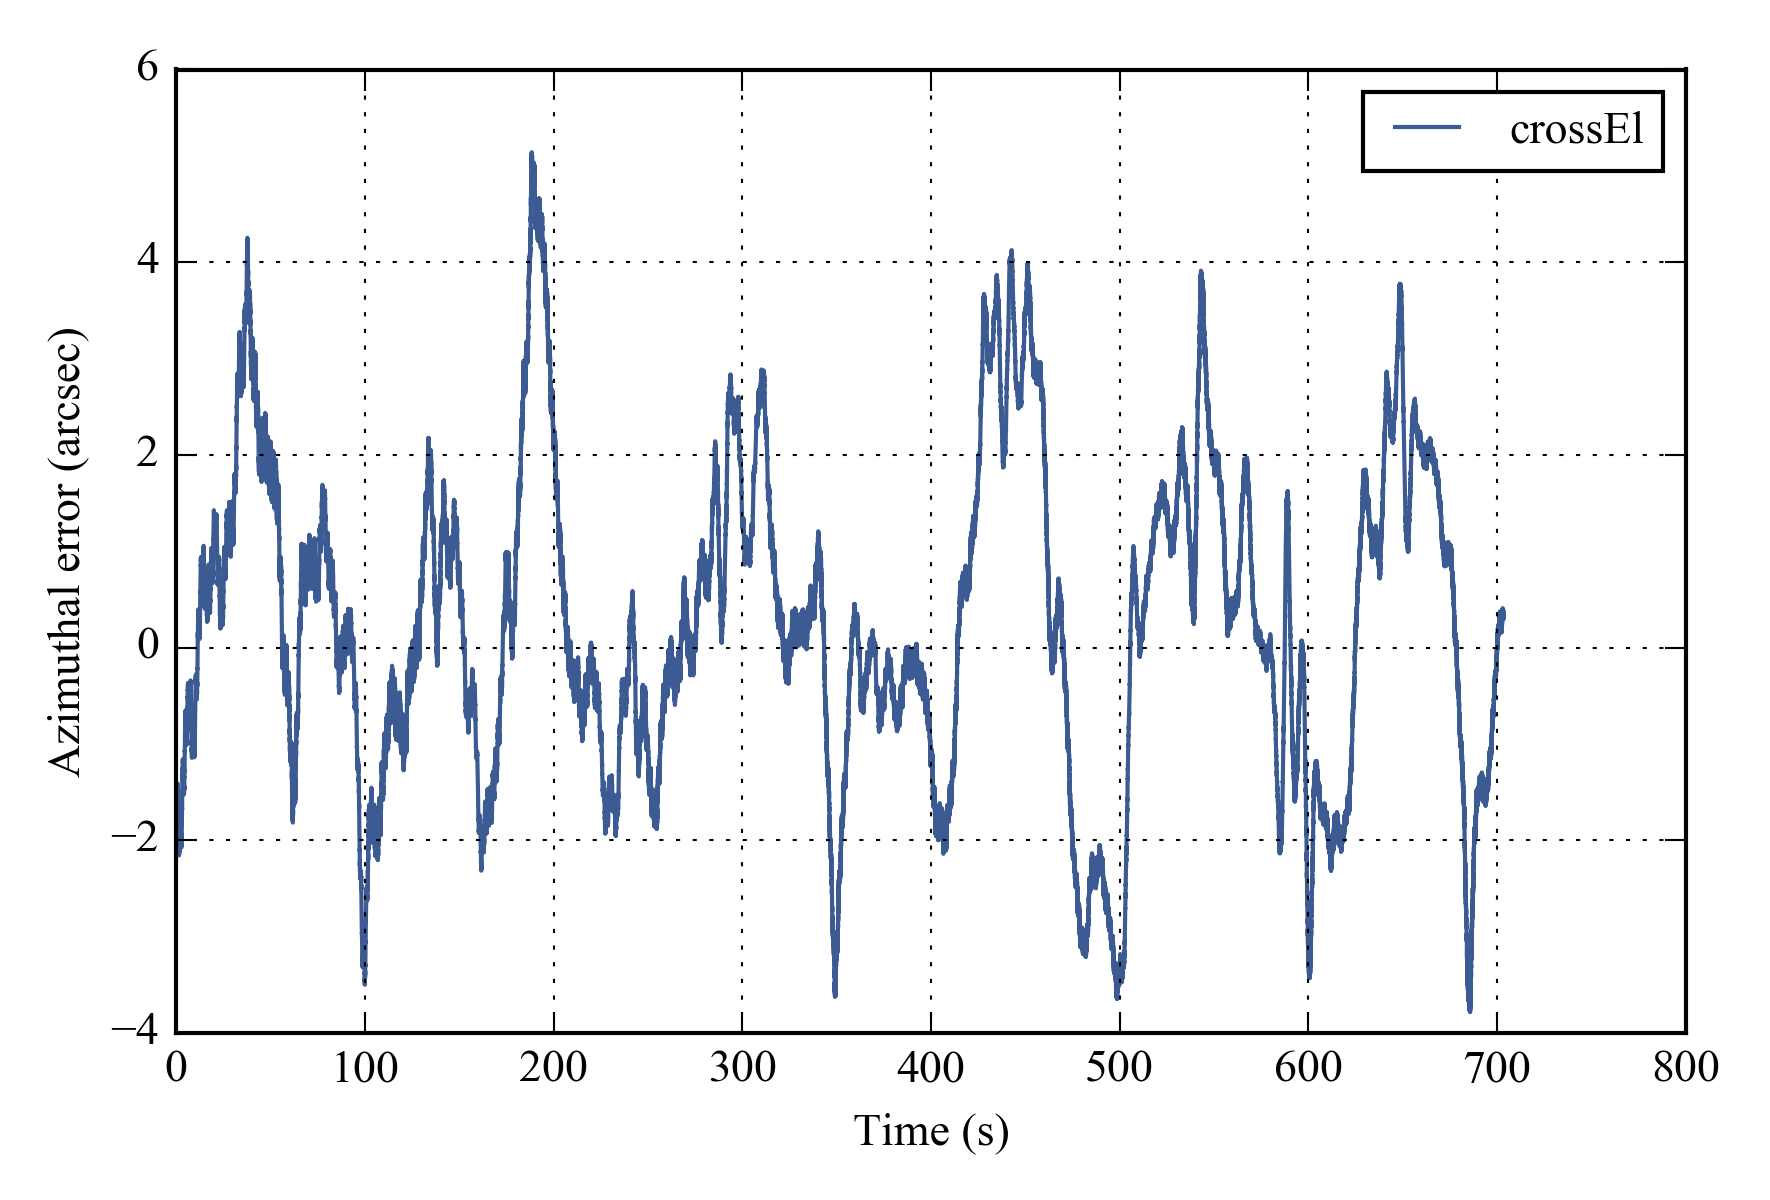
\includegraphics{Figures/simplePlot_crossEl.png}
\vspace{-0.5cm}
\caption[Cross-elevation error indoors]{Cross-elevation error indoors.}
\label{fig:simplePlot_crossEl}
\end{center}
\end{figure}

Note that this behavior also implies the momentum dump loop working well. While we do not have the data to show due a mistake in the archiving software, the CCMG gimbal angle was staying for all this time within a few degrees of zero, and has being working consistently well for multiple months before this writing. This has allowed us to always maintain the gimbal in the middle of the range, and ensured long-term stability.

\subsection{On-sky pointing control}


On-sky, lifted pointing test is the ultimate test that we can run from the ground without having the optics in place. We show two sets of data; the first one (configuration 1) was taken with the star camera positioned at $\sim\SI{43}{\degree}$ elevation at the very end of the BETTII boom (pointing in the $(\vectors{y}, \vectors{z})$ plane). This gave access to a large patch of sky, as the boom could be almost sticking out through the high bay door. The second set (configuration 2) features the star camera installed at a temporary $\sim\SI{23}{\degree}$ angle from horizontal in the $(\vectors{x}, \vectors{z})$ plane. This configuration is more similar to the final flight configuration where it will be at a nominal \SI{45}{\degree} from horizontal in that same plane. Putting it at an elevation of $\sim\SI{23}{\degree}$ angle allows coverage of a reasonable patch of sky, although it remains very constraining.

\begin{landscape}
\begin{figure}[!h]
\begin{subfigure}[b]{0.7\textwidth}
		\centering
		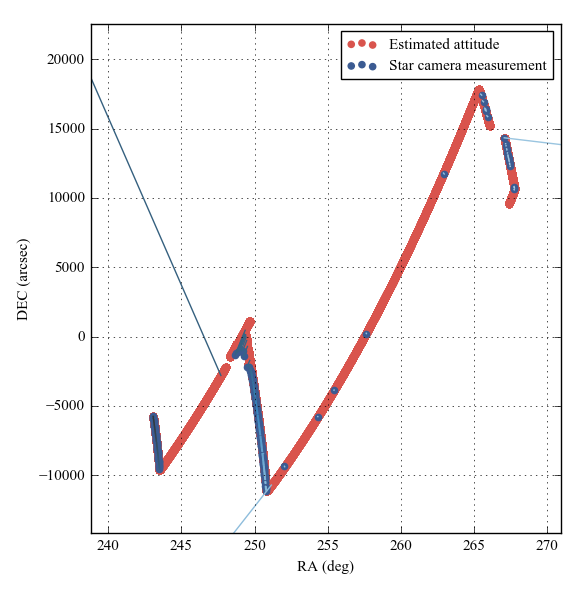
\includegraphics[width=0.98\textwidth]{Figures/Slew_with_starcam_1.png} 
		\caption{}
		\label{subfig:SlewWithStarcam1}
\end{subfigure}
\begin{subfigure}[b]{0.7\textwidth}
		\centering
		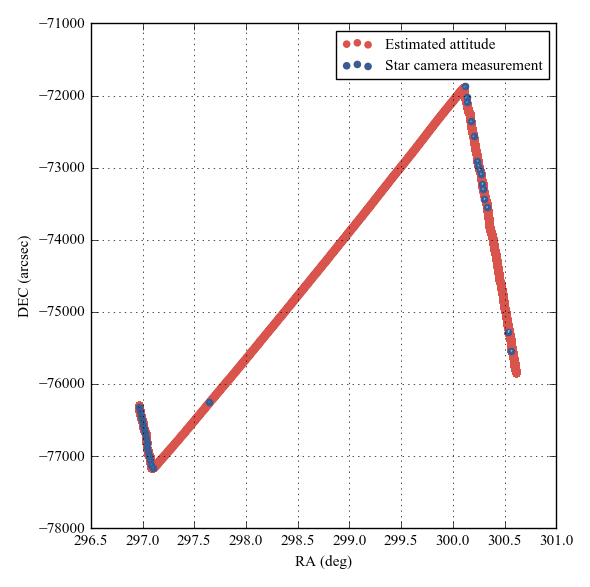
\includegraphics[width=0.98\textwidth]{Figures/Slew_with_starcam_2.png} 
		\caption{}
		\label{subfig:SlewWithStarcam2}
\end{subfigure}
\caption[Slew and point on the sky]{Slew and point on the sky. (\subref{subfig:SlewWithStarcam1}): Two consecutive slews with the camera in configuration~1 totalling $\sim\SI{25}{\degree}$ in azimuth. The time flows from left to right on this graph. (\subref{subfig:SlewWithStarcam2}): Point, slew and point with the camera in configuration~2. The low rate of star camera solutions towards the end of the run is due to increased cloud coverage and increased surrounding light in the very early morning.}
\label{fig:SlewWithStarcam}
\end{figure}
\end{landscape}

In Fig.~\ref{fig:SlewWithStarcam} we show two typical pointing runs during a night in June~2016. That night marked the transition to configuration 2 and a reorganization of the high bay to accommodate rotating the payload so that it faces the door, and so that the telescopes can see out of the door.

For the first run that night, shown on Fig.~\ref{fig:SlewWithStarcam}\subref{subfig:SlewWithStarcam1}, we tested the new gyroscope mount, new algorithms, and new flight procedures. The run shows two consecutive slews (the swathes with little to no star camera solutions) spanning a total of about \SI{25}{\degree} in RA. Note that the scales are different in RA and DEC for display convenience. There are two noticeable features to this figure. The first is that some star camera solutions appear to be false positive, a result from non-optimal star camera parameters which involved too few stars required to confirm a match. This can be easily fixed by increasing this parameter.

The second, and more concerning problem is the apparent drift of the star camera solution after the first slew. This is what made us realize that correcting for biases only was not capturing the entire behavior of the gyroscope-star camera system pair. We interpret the resulting large error at the end of the first slew as a misalignment between the star camera orientation and the 3D gyroscope mount, and have developed flight software to properly estimate this out (see Chapter~\ref{chap:controls}, Section~\ref{subsec:enhancedKalman}).

If this is a problem during flight, we anticipate resetting the estimator's position each time we finish slewing, to restart the Kalman filter using the original biases.

The second run of the night, which was also our first run in configuration 2, does not exhibit this behavior, partly due to a better alignment between the gyros and the star camera, and also because the slew is half as long as the first slew in the other picture. 

For this second run, we show the pointing stability in cross-elevation in Fig.~\ref{fig:crossEl_outside}. This picture is to be compared with the test done indoors, showed in Fig.~\ref{fig:simplePlot_crossEl}. Here the peak-to-peak errors are increased by a factor of $\sim 5$, but the r.m.s deviation is still $\le\ang{;;5}$. This satisfies the $\pm\ang{;;15}$ requirement for more than 95\% of the points, which is very encouraging.
\begin{figure}[!h]
\begin{center}
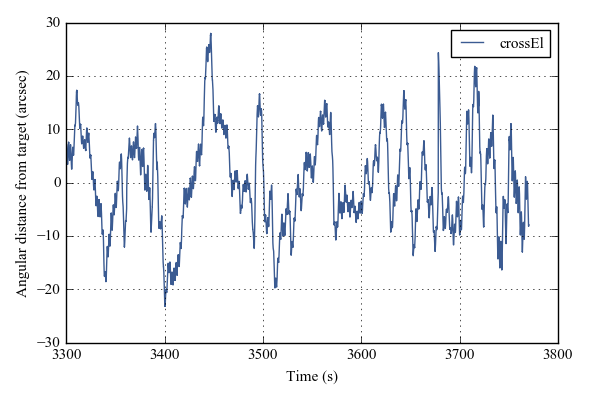
\includegraphics{Figures/crossEl_outside.png}
\vspace{-0.5cm}
\caption[Cross-elevation error]{Cross-elevation error for a test on the sky (see text for description).}
\label{fig:crossEl_outside}
\end{center}
\end{figure}

Another view at the pointing stability is proposed in Fig.~\ref{fig:simple2DPlot_crossEl_elevation}, which presents the data as a 2D plot of the error in both elevation and cross-elevation, augmented by a 2D Kernel density contour plot to better show where the density peak lies. Note that contours are separated linearly, so that data is 10 times more likely to be inside the brightest contour than outside the black outer contour. The values of the contours are not meaningful, since they refer to lines of same probability density, which doesn't easily relate to a percentile value. 

The striking asymmetry of this plot reveals that the elevation control is, for now, much more accurate than the cross-elevation loop, which is to be expected due to the much lower inertia of the rotators (at the time of this run, the mirrors were not installed on the rotators). We expect degradation of the elevation accuracy once the siderostats are mounted on the rotators, even after tuning the PID gains.

\begin{figure}[!h]
\begin{center}
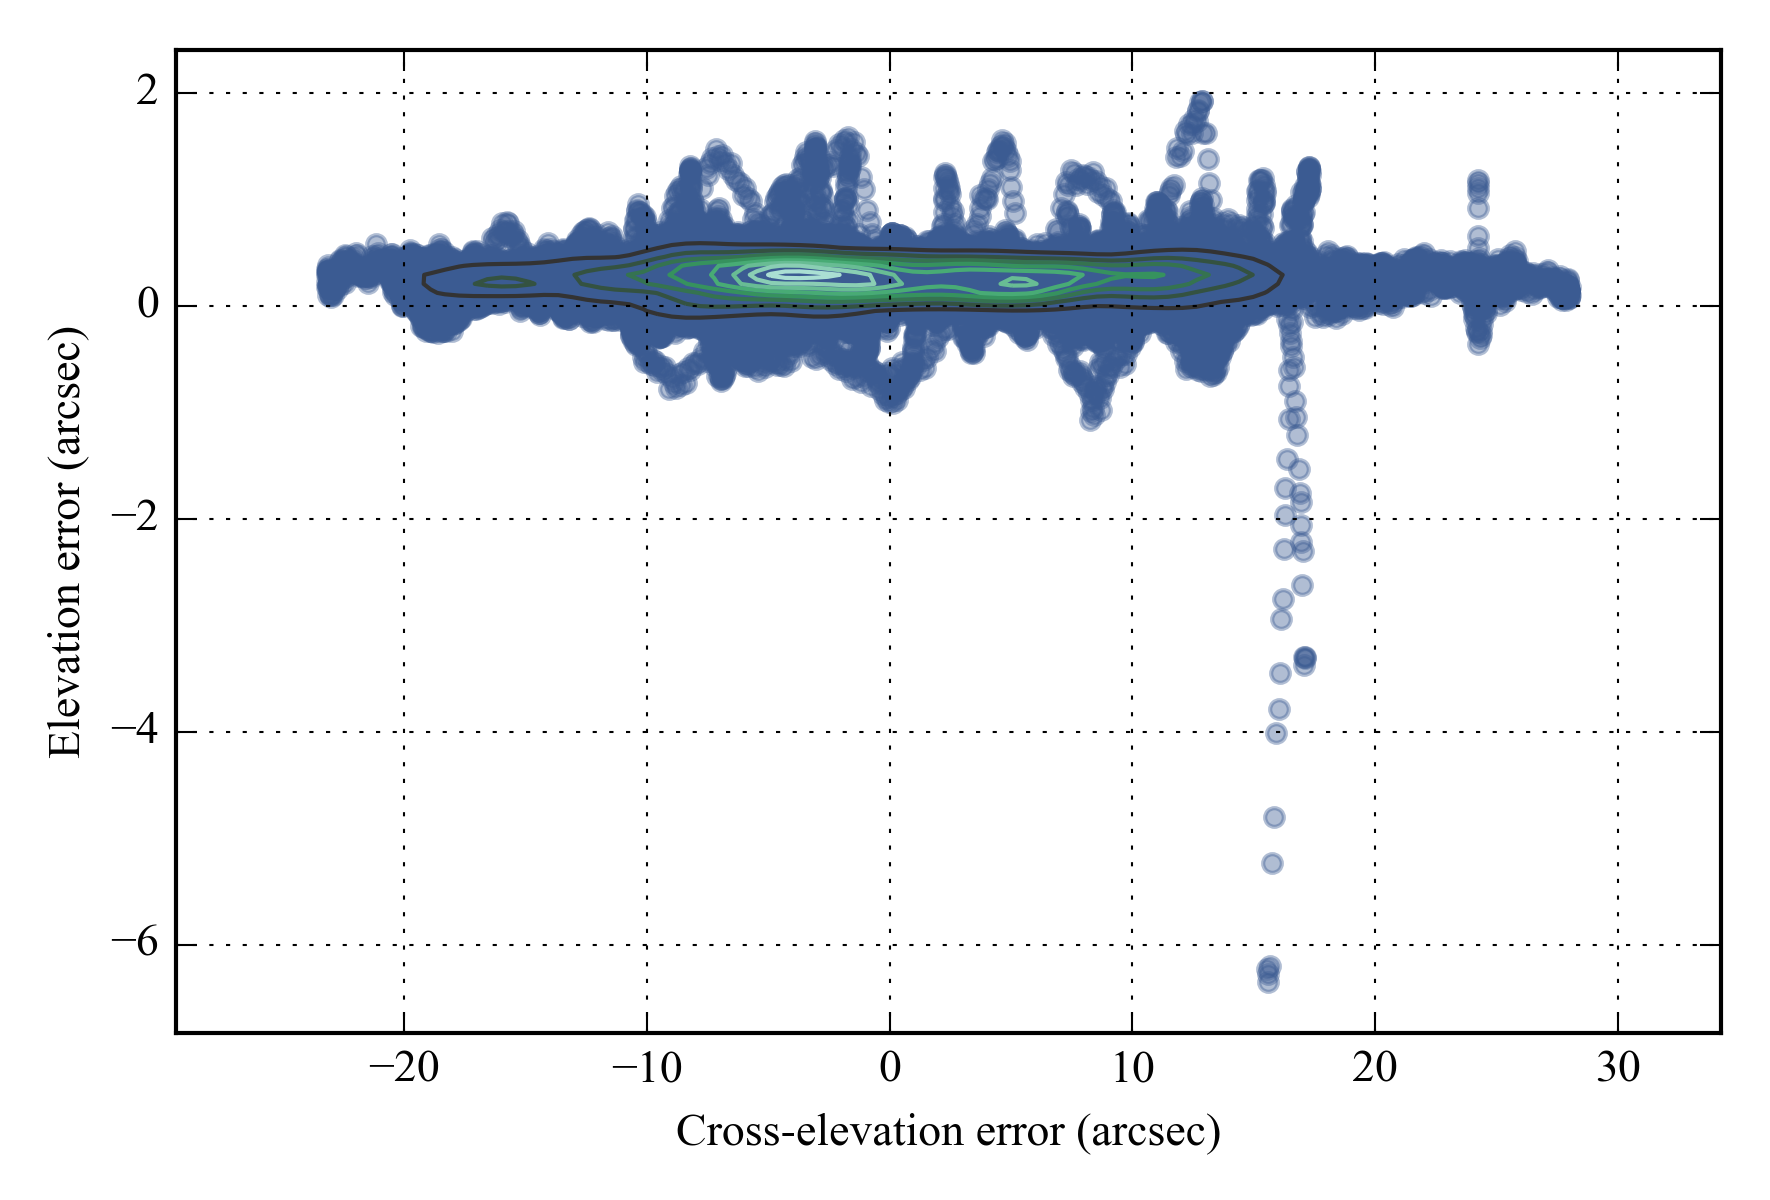
\includegraphics{Figures/simple2DPlot_crossEl_elevation.png}
\vspace{-0.5cm}
\caption[Elevation and cross-elevation error]{Elevation and cross-elevation error for a test on the sky.}
\label{fig:simple2DPlot_crossEl_elevation}
\end{center}
\end{figure}




\subsection{What's left: Fine guiding sensor loop implementation}

The last on-sky pointing tests have consistently shown:
\begin{enumerate}
\item our ability to always know where we are pointed using a robust star camera solution
\item our ability to slew large amounts while maintaining the wheels close to their zero position (which indicates a successful momentum dumping loop)
\item our ability to keep the telescope vector pointed to an inertial target to within the specificied $\pm\ang{;;15}$ more a large fraction of the time
\item our ability to have small attitude errors which can be fed to the delay line for further correction
\end{enumerate}

However, despite this relative success, one key item has yet to be implemented before flight: the fine guiding loop, which brings both beams to overlap better than $\ang{;;1.5}$. In order to be implemented, the optics, cryostat, and tip/tilt mechanisms all have to be integrated into the payload in order to make it function.

We have started planning for this upcoming integration by designing a C++ software to handle the task at hands. In this section we present the notional architecture for this last piece of software, but warn the reader that many unknowns will remain until the optics are installed in the truss. In particular, our main concern lies in the transition mode that we called "ACQUIRE", which might require a lot of tuning. 

The role of the fine guiding loop is to use the fine guiding sensor (FGS, an H1RG detector with two window readouts, one for each arm) to determine the centroid of a known source within the field of view. The location of this source on each of the readout windows of the detector (each window shows what is seen by each arm) will then be compared to known pixel locations that ensure overlap between the two science beams. The errors signals are then $\Delta x_L$, $\Delta y_L$, $\Delta x_R$, $\Delta y_R$, where the subscripts designate the left and right arm, respectively. These error signals are rotated to the proper reference frame and fed to the tip/tilt mechanisms, which zeroes them out very quickly thanks to their very large actuation bandwidth and very small inertia. 

Since the errors are zeroed out almost instantaneously, these errors signals cannot be used to determine the attitude of the entire payload. However, the angular deviation of each tip/tilt stage from their nominal position has information about the overall pointing error of the truss. To illustrate this feature, let's suppose that both windows are perfectly aligned and the detector axes (X,Y) match the elevation and cross-elevation, respectively. In this case, if both tip/tilt stage need to correct for a positive elevation error, it means that the entire truss is mispointed in elevation. Similarly, if the cross-elevation correction happens in the same direction, it means that a movement of the truss in cross-elevation will correct it and bring the tip/tilt stages to their nominal position.

We can generalize this statement by saying that the common-mode deviations from the nominal position of the tip/tilt stages represent an estimator for the attitude difference between the payload and the guide star. This information is processed, rotated in the correct reference frame, an injected into the Kalman filter estimator in replacement of a star camera measurement. The weight (or variance) of this new measurement is considerably smaller than the star camera, since it is the most trusted attitude measurement that we can have. 

At full speed and sampling only \ang{;;15}$\times$\ang{;;15} windows, the fine guiding loop can provide these absolute position estimates at \SI{50}{\hertz}. 

There are many challenges with this system. The first is to robustly, autonomously identify the chosen guide star within the field of view. For this, we design a blob-finding software which examines the images received from the fine guiding sensor and identifies the brightest $N$ blobs in the image. The targets are carefully chosen so that the guide stars are the brightest sources in the image, which enhances the chances of finding the correct star. 

ACQUIRE mode involves progressively reducing the size of the FOV in the fine guiding sensor, starting with a $\ang{;5;}\times\ang{;5;}$ FOV at \SI{2}{\second} per frame, down to \ang{;;15}$\times$\ang{;;15} at \SI{50}{\hertz}. 

%\section{	Conclusion and status of implementation}